\documentclass[11pt,a4paper]{article}
\usepackage[utf8]{inputenc}
\usepackage[T1]{fontenc}
\usepackage{lmodern}
\usepackage{amsmath,amssymb,mathtools}
\usepackage[margin=2.2cm]{geometry}
\usepackage{microtype}
\usepackage{booktabs,array,tabularx}
\usepackage{enumitem}
\usepackage{xcolor}
\usepackage[most]{tcolorbox}
\usepackage{listings}
\usepackage{graphicx}
\usepackage{tikz}
\usetikzlibrary{arrows.meta,positioning}
\usepackage[colorlinks=true,linkcolor=blue!60!black,urlcolor=blue!60!black]{hyperref}
\usepackage{fancyhdr}
\setlength{\parindent}{0pt}
\setlength{\parskip}{6pt}
\renewcommand{\arraystretch}{1.25}
\pagestyle{fancy}
\fancyhf{}
\fancyhead[L]{\small GATE DA 2027 --- Programming, DSA (Deep)}
\fancyhead[R]{\small Ramu \& Somu Notes}
\fancyfoot[C]{\thepage}

\newcommand{\Oh}{\mathcal{O}}
\newcommand{\py}[1]{\texttt{#1}}

% ---------- code listings ----------
\lstdefinestyle{py}{language=Python,basicstyle=\ttfamily\small,keywordstyle=\color{blue!60!black}\bfseries,
  commentstyle=\color{green!40!black}\itshape,stringstyle=\color{red!55!black},
  backgroundcolor=\color{gray!9},frame=single,rulecolor=\color{gray!40},breaklines=true,
  showstringspaces=false,columns=fullflexible,aboveskip=4pt,belowskip=2pt,
  xleftmargin=2pt,xrightmargin=2pt}
\lstdefinestyle{out}{basicstyle=\ttfamily\small,backgroundcolor=\color{yellow!10},frame=single,
  rulecolor=\color{orange!40},breaklines=true,showstringspaces=false,columns=fullflexible,
  aboveskip=0pt,belowskip=4pt,xleftmargin=2pt,xrightmargin=2pt}
\lstset{style=py}

% ---------- boxes ----------
\newtcolorbox{story}[1][]{breakable,enhanced,colback=yellow!10,colframe=orange!80!black,
  fonttitle=\bfseries,title={Ramu \& Somu: #1},left=6pt,right=6pt,top=4pt,bottom=4pt}
\newtcolorbox{formula}[1][Key facts]{breakable,enhanced,colback=blue!5,colframe=blue!60!black,
  fonttitle=\bfseries,title={#1},left=6pt,right=6pt}
\newtcolorbox{example}[1][Worked example]{breakable,enhanced,colback=green!6,colframe=green!45!black,
  fonttitle=\bfseries,title={#1},left=6pt,right=6pt}
\newtcolorbox{trap}{breakable,enhanced,colback=red!5,colframe=red!60!black,
  fonttitle=\bfseries,title={Common GATE traps},left=6pt,right=6pt}
\newtcolorbox{intuition}{breakable,enhanced,colback=gray!8,colframe=gray!60!black,
  fonttitle=\bfseries,title={Idea in plain words},left=6pt,right=6pt}

\title{\Huge\bfseries GATE DA 2027\\[4pt] \Large Programming, Data Structures and Algorithms\\[2pt]\large\emph{Deep Edition: from arithmetic to interview patterns, with Mermaid maps and 2024--2026 past questions}\\[8pt]
\large Python, core data structures, searching and sorting,\\divide-and-conquer and basic graph algorithms\\
with the stories of Ramu and Somu}
\author{}
\date{}

\begin{document}
\maketitle
\thispagestyle{empty}

\begin{center}
\begin{tcolorbox}[colback=yellow!10,colframe=orange!80!black,width=0.9\textwidth,breakable]
\textbf{Ramu and Somu once more.}\\
\textbf{Ramu} asks ``but why?'' about everything. \textbf{Somu} explains with small everyday stories: library shelves, queues at a canteen, a phone contact list, a town's roads.\\[4pt]
\textbf{Syllabus covered (GATE DA, Section 4):} Python programming; core data structures (stacks, queues, linked lists, trees, hash tables); searching (linear and binary); sorting (selection, bubble, insertion, merge, quick); divide-and-conquer; introduction to graph theory; basic graph algorithms (traversals and shortest paths).\\[4pt]
\textbf{How the book is organised.} Part I builds foundations from addition and division up to recursion. Part II is the full subject (Python, data structures, searching, sorting, divide-and-conquer, graphs). Part III is a gallery of Mermaid maps. Part IV solves the previous GATE DA questions of 2024, 2025 and 2026 one by one. Part V trains Google-style interview patterns. \textbf{Every code example was actually run} and outputs shown are real.
\end{tcolorbox}
\end{center}

\tableofcontents
\newpage

% =====================================================================
\part{Foundations: from arithmetic to thinking like a programmer}

\section{Numbers, Operators and What the Computer Really Does}
\begin{story}[Why start with $7+3$?]
Ramu: ``Somu, GATE asks about quicksort and graphs. Why are we starting with addition?''\\
Somu: ``Because almost every wrong answer in a coding question is an arithmetic detail: $-7\,//\,2$, a float that is not exactly $0.3$, or an operator that binds tighter than you thought. If the basement is shaky, the tower falls. We go slowly here, then speed up.''
\end{story}

\subsection{The six arithmetic operators of Python}
\begin{formula}[Operators, with the meaning in everyday words]
\begin{tabularx}{\textwidth}{llX}
\toprule
Operator & Example $\to$ result & Meaning\\\midrule
\py{+} addition & \py{7+3} $\to$ \py{10} & total of two quantities\\
\py{-} subtraction & \py{7-3} $\to$ \py{4} & difference, ``how far from''\\
\py{*} multiplication & \py{7*3} $\to$ \py{21} & repeated addition\\
\py{/} true division & \py{7/2} $\to$ \py{3.5} & always gives a \emph{float}\\
\py{//} floor division & \py{7//2} $\to$ \py{3} & divide, then round \emph{down}\\
\py{\%} remainder (modulo) & \py{7\%2} $\to$ \py{1} & what is left over\\
\py{**} power & \py{2**10} $\to$ \py{1024} & repeated multiplication\\\bottomrule
\end{tabularx}

\medskip
\textbf{Link between the three division operators:} for integers $a,b$ ($b\neq 0$), \quad $a = b\cdot(a\,//\,b) + (a\,\%\,b)$.
\end{formula}

\begin{story}[Division is sharing sweets]
Somu has 7 sweets for 2 friends. \py{7//2} $=3$ each (the \emph{quotient}); \py{7\%2} $=1$ sweet is left (the \emph{remainder}); \py{7/2} $=3.5$ is what each gets if you may cut the last sweet.\\
Ramu: ``And with negative numbers?'' Somu: ``Floor means \emph{toward minus infinity}, not toward zero. So \py{-7//2} is $-4$, because $-3.5$ rounded down is $-4$. Then the identity forces \py{-7\%2}$=-7-2(-4)=1$.''
\end{story}

\begin{example}[Floor division and modulo with negative numbers (real output)]
\begin{lstlisting}
print(-7//2, -7%2, 7//-2, 7%-2, divmod(-7,2))
\end{lstlisting}
\begin{lstlisting}[style=out]
-4 1 -4 -1 (-4, 1)
\end{lstlisting}
Check the identity for \py{7//-2 = -4} and \py{7\%-2 = -1}: $(-2)(-4)+(-1)=8-1=7$. \checkmark\ 
\textbf{Rule:} in Python, \py{a\%b} always has the sign of \py{b}. (In C it follows the sign of \py{a}; GATE questions in Python follow Python.)
\end{example}

\subsection{Order of evaluation (precedence)}
Ramu: ``Why is $2+3\cdot 4^2=50$ and not 400?'' Because \py{**} binds tightest, then \py{* / // \%}, then \py{+ -}, then comparisons, then \py{not}, \py{and}, \py{or}. Parentheses override everything.
\begin{lstlisting}
print(2+3*4**2, (2+3)*4**2, -2**2, 2**3**2)
\end{lstlisting}
\begin{lstlisting}[style=out]
50 80 -4 512
\end{lstlisting}
Two classic surprises: \py{-2**2} is $-(2^2)=-4$ because \py{**} is stronger than unary minus; and \py{2**3**2} is $2^{(3^2)}=2^9=512$ because \py{**} associates from the \emph{right}.

\subsection{Integers have no size limit; floats do}
Python integers grow as needed, so \py{2**100} is exact. Floats store about 15--16 decimal digits in binary, and most decimals (like $0.1$) have no finite binary form, exactly as $1/3$ has no finite decimal form.
\begin{lstlisting}
print(10**20+1, 2**100)
print(0.1+0.2, 0.1+0.2==0.3, abs((0.1+0.2)-0.3)<1e-9)
\end{lstlisting}
\begin{lstlisting}[style=out]
100000000000000000001 1267650600228229401496703205376
0.30000000000000004 False True
\end{lstlisting}
\begin{trap}
Never test floats with \py{==}; compare with a tolerance. Also \py{round(2.5)=2} and \py{round(3.5)=4}: Python rounds halves to the nearest \emph{even} number (``banker's rounding''), while \py{int(-2.7)=-2} truncates toward zero, unlike floor.
\end{trap}

\subsection{Binary numbers and bit operations}
Computers count in base 2. Position $k$ (from the right, starting at 0) is worth $2^k$. So $1101_2 = 8+4+0+1 = 13$.
\begin{formula}[Bit tricks worth remembering]
\begin{itemize}[leftmargin=*,itemsep=1pt]
\item \py{x<<k} multiplies by $2^k$; \py{x>>k} is \py{x//2**k}.
\item \py{x\&1} is $1$ iff $x$ is odd. \py{x\&(x-1)} clears the lowest set bit.
\item Number of binary digits of $n\ge1$ is $\lfloor\log_2 n\rfloor+1$. For $n=1000$: $\lfloor 9.97\rfloor+1=10$ (this is exactly the idea behind 2026 Q31, solved later).
\item \py{\^} is XOR: equal bits give 0, different bits give 1.
\end{itemize}
\end{formula}
\begin{lstlisting}
print(bin(13), int("1101",2), 13>>1, 13<<2, 13&6, 13|6, 13^6)
print(len(str(2**100)), bin(255).count("1"), 255 .bit_length())
\end{lstlisting}
\begin{lstlisting}[style=out]
0b1101 13 6 52 4 15 11
31 8 8
\end{lstlisting}

\subsection{Truth values and short-circuit logic}
\py{and}, \py{or} do not return just \py{True}/\py{False}; they return one of their operands. \py{x and y} returns \py{x} if \py{x} is falsy, else \py{y}. \py{x or y} returns \py{x} if \py{x} is truthy, else \py{y}. Falsy values: \py{0, 0.0, "", [], \{\}, None, False}. Python evaluates left to right and \emph{stops early} (short-circuit): \py{x != 0 and 10/x > 1} never divides by zero.
\begin{lstlisting}
print(5>3>1, 5>3>4, not 0, 3 and 0, 3 or 0, [] or "x")
\end{lstlisting}
\begin{lstlisting}[style=out]
True False True 0 3 x
\end{lstlisting}
Chained comparison \py{5>3>1} means \py{5>3 and 3>1}.

\section{Variables, References and Mutability}
\begin{story}[A name is a label, not a box]
Ramu: ``If I write \py{b = a}, did Python copy the list?'' Somu: ``No. A variable is a sticky label on an object. \py{b = a} sticks a \emph{second label} on the \emph{same} object. Numbers and strings cannot be changed in place (immutable), so changing one makes a new object and moves the label. A list can be changed in place (mutable), so every label sees the change.''
\end{story}
\begin{lstlisting}
a=[1,2,3]; b=a; c=a[:]; b.append(4); print(a,c,a is b,a is c)
x=10; y=x; y+=1; print(x,y)
t=(1,[2,3]); t[1].append(4); print(t)
\end{lstlisting}
\begin{lstlisting}[style=out]
[1, 2, 3, 4] [1, 2, 3] True False
10 11
(1, [2, 3, 4])
\end{lstlisting}
The tuple is immutable, but it \emph{holds} a mutable list, and the list can still grow. This single idea explains three GATE-style traps: aliasing, the shared default argument (2026 Q16) and the closure that keeps its own list (2026 Q50).

\begin{center}
\includegraphics[width=0.98\textwidth]{d2.pdf}
\end{center}

\section{Reading Code Like a Machine: Tracing and Loop Invariants}
Somu's method for any output question has four steps: (1) write the variables as a table; (2) execute line by line, updating the table; (3) stop and look for a pattern as soon as the table repeats; (4) re-check the edge case ($n=0$, $n=1$, empty list).

\begin{example}[Sum of the first $n$ numbers three ways]
\begin{lstlisting}
print(sum(range(1,101)), sum(i*i for i in range(1,6)))
\end{lstlisting}
\begin{lstlisting}[style=out]
5050 55
\end{lstlisting}
Gauss's formula $\frac{n(n+1)}2=5050$; the squares give $1+4+9+16+25=55=\frac{n(n+1)(2n+1)}{6}$ at $n=5$. When a loop looks like a sum, try a formula; GATE loves loops whose total is a closed form.
\end{example}

\begin{intuition}
\textbf{Loop invariant.} A statement that is true before the loop, stays true after every iteration, and, combined with the exit condition, proves the answer. For binary search: ``if the target exists, it lies in \py{a[lo..hi]}''. For insertion sort: ``\py{a[0..k-1]} is sorted''. Naming the invariant turns a scary loop into two small checks.
\end{intuition}

\section{Functions, Recursion and the Call Stack}
A function call creates a fresh workspace (a \emph{frame}) holding its parameters and local variables. Frames are stacked; the newest sits on top, and returning pops it. Recursion is just a function calling itself with a smaller input, and it needs two parts: a \textbf{base case} (stops) and a \textbf{recursive case} (moves toward the base).

\begin{center}
\includegraphics[width=0.8\textwidth]{d9.pdf}
\end{center}

\begin{example}[Fast exponentiation: $3^{13}$ in about $\log_2 13$ multiplications]
\begin{lstlisting}
def power(b,e):
    if e==0: return 1
    h=power(b,e//2)
    return h*h if e%2==0 else h*h*b
print(power(3,13), 3**13)
\end{lstlisting}
\begin{lstlisting}[style=out]
1594323 1594323
\end{lstlisting}
\textbf{Why it works:} $b^e=(b^{e/2})^2$ when $e$ is even and $b\cdot(b^{(e-1)/2})^2$ when odd. The exponent halves each call, so the depth is $\lfloor\log_2 e\rfloor+1$. This ``halve the problem'' pattern returns in binary search, merge sort and the 2026 question on repeated halving.
\end{example}

\begin{example}[Euclid's gcd, the oldest algorithm]
\begin{lstlisting}
def gcd(a,b):
    while b: a,b=b,a%b
    return a
print(gcd(48,18))
\end{lstlisting}
\begin{lstlisting}[style=out]
6
\end{lstlisting}
Trace: $(48,18)\to(18,12)\to(12,6)\to(6,0)$. Why: any number dividing both $a$ and $b$ also divides $a\bmod b$, so the pair shrinks without changing the answer.
\end{example}

\section{Strings, Lists, Dicts and Comprehensions in One Page}
\begin{lstlisting}
print(sorted("banana"), "banana".count("a"), "banana"[::-1], "banana"[1:4])
print([i for i in range(10) if i%3==0], {i:i*i for i in range(4)}, {x%3 for x in range(10)})
d={}
for w in "to be or not to be".split(): d[w]=d.get(w,0)+1
print(d)
\end{lstlisting}
\begin{lstlisting}[style=out]
['a', 'a', 'a', 'b', 'n', 'n'] 3 ananab ana
[0, 3, 6, 9] {0: 0, 1: 1, 2: 4, 3: 9} {0, 1, 2}
{'to': 2, 'be': 2, 'or': 1, 'not': 1}
\end{lstlisting}
Slicing \py{s[i:j]} takes positions $i,\dots,j-1$ (the end is excluded) and \py{s[::-1]} reverses. A dict counts words in $O(1)$ average per word: this ``count with a dictionary'' idiom reappears in almost every interview problem.

\section{Thinking About Cost: How Big Can $n$ Be?}
\begin{center}
\includegraphics[width=0.9\textwidth]{d1.pdf}
\end{center}
A machine does roughly $10^8$ simple operations per second. So $n=10^5$ with an $O(n^2)=10^{10}$ algorithm takes minutes, but $O(n\log n)\approx 1.7\times10^6$ takes milliseconds. Reading the constraints first tells you which algorithm family to reach for; this habit is what interviewers (Google included) test hardest.

\part{The Full Subject, Step by Step}
\section{Python Programming}

\begin{story}[The calculator that does not lie]
Ramu is learning to program and tries \py{-7 // 2} on Python. He expects $-3$ (``three and a half, drop the half''). Python says $-4$. Somu explains: \py{//} is \emph{floor} division: it rounds towards $-\infty$, not towards zero. And Python's \py{\%} then has the \emph{sign of the divisor}, so that $a=(a//b)\cdot b+(a\%b)$ always holds: $-7=(-4)(2)+1$. GATE loves such details because they are easy to get wrong when you are in a hurry.
\end{story}

\subsection{Basic types and operators}
\begin{center}
\begin{tabularx}{\textwidth}{>{\raggedright\arraybackslash}p{2.6cm} >{\raggedright\arraybackslash}p{3.2cm} c >{\raggedright\arraybackslash}X}
\toprule
\textbf{Type} & \textbf{Example} & \textbf{Mutable?} & \textbf{Notes}\\
\midrule
\py{int} & \py{42} & no & unlimited precision\\
\py{float} & \py{2.5} & no & 64-bit; \py{round(2.5)} is \py{2} (round half to even)\\
\py{bool} & \py{True} & no & subclass of int; \py{True+True} is \py{2}\\
\py{str} & \py{"GATE"} & no & immutable; slicing makes a new string\\
\py{tuple} & \py{(1,2)}, \py{(1,)} & no & single element needs a trailing comma\\
\py{list} & \py{[1,2,3]} & \textbf{yes} & ordered, any items\\
\py{set} & \py{\{1,2\}} & yes & unique items, no order, hashable items only\\
\py{dict} & \py{\{'a':1\}} & yes & key $\to$ value; keys must be hashable\\
\bottomrule
\end{tabularx}
\end{center}

\begin{formula}[Operators you must be fluent with]
\begin{itemize}[noitemsep]
\item \py{/} true division (always \py{float}); \py{//} floor division; \py{\%} modulo; \py{**} power (right associative: \py{2**3**2} is $2^{9}=512$).
\item \py{7//2}$=3$, \py{-7//2}$=-4$, \py{7\%3}$=1$, \py{-7\%3}$=2$, \py{5\%-3}$=-1$, \py{divmod(17,5)}$=(3,2)$.
\item Comparison chains work as in maths: \py{3>2>1} is \py{True}, \py{3>2>2} is \py{False}.
\item \py{==} compares values; \py{is} compares identity (same object). \py{[1]==[1]} is \py{True} but \py{[1] is [1]} is \py{False}.
\item \textbf{Truthiness:} empty things and zero are false: \py{bool([])}, \py{bool(0)} are \py{False}; \py{bool("0")} and \py{bool(" ")} are \py{True} (non-empty strings).
\item Logical operators short-circuit: in \py{a and b}, if \py{a} is false \py{b} is never evaluated; \py{x or y} returns the first truthy operand.
\end{itemize}
\end{formula}

\begin{lstlisting}
print(7//2, -7//2, 7%3, -7%3, 2**3**2, 10/4, 10//4)
print(bool([]), bool(0), bool("0"), bool(" "))
print([1]==[1], [1] is [1])
\end{lstlisting}
\begin{lstlisting}[style=out]
3 -4 1 2 512 2.5 2
False False True True
True False
\end{lstlisting}


\subsection{Mutable vs immutable objects}
\begin{story}[Whiteboard and printed photo]
Ramu has a \textbf{whiteboard} and a \textbf{printed photo}. The whiteboard is \emph{mutable}: erase a word, write another, and it is still the same whiteboard. The printed photo is \emph{immutable}: to make it look different you must print a brand-new photo, and the old one stays exactly as it was. In Python, every value is such an object; the only question is whether it can be edited \emph{in place}.
\end{story}
\begin{formula}[Definition and the two groups]
\textbf{Mutable} = can be changed in place after creation: \py{list}, \py{dict}, \py{set}, most user-defined class objects.\\
\textbf{Immutable} = cannot be changed after creation (any ``change'' builds a new object): \py{int}, \py{float}, \py{bool}, \py{str}, \py{tuple}, \py{frozenset}, \py{None}.\\
\textbf{Quick test:} if an operation changes the object itself (\py{append}, \py{sort}, \py{pop}, \py{x[i]=...}) the type is mutable; if every operation returns a new value (\py{s.upper()}, \py{x+1}) it is immutable.
\end{formula}
\begin{lstlisting}
a = [1, 2, 3]; a[0] = 99; print(a)          # list edited in place
s = "GATE"
try:
    s[0] = "X"
except TypeError as e:
    print("TypeError:", e)
t = "X" + s[1:]                              # builds a NEW string
print(s, t, id(s) == id(t))

l = [1, 2]; i1 = id(l); l.append(3); print(id(l) == i1)   # same object
n = 5;      i2 = id(n); n += 1;      print(id(n) == i2)   # new object
\end{lstlisting}
\begin{lstlisting}[style=out]
[99, 2, 3]
TypeError: 'str' object does not support item assignment
GATE XATE False
True
False
\end{lstlisting}
\begin{formula}[Why it matters (all of these are GATE favourites)]
\begin{itemize}[noitemsep]
\item \textbf{Aliasing:} \py{b = a} copies nothing. For a list, a change through \py{b} is visible through \py{a}; for an \py{int} or \py{str} no such effect is possible. (See the aliasing examples below.)
\item \textbf{Function arguments:} a function can mutate a list argument in place (caller sees it); rebinding the parameter name (\py{lst = [9]}) does not affect the caller.
\item \textbf{Mutable default argument:} \py{def f(x, L=[])} reuses one list for every call.
\item \textbf{Hashing:} dictionary keys and set elements must be immutable (hashable). \py{\{[1,2]: 'no'\}} raises \py{TypeError: unhashable type: 'list'}; \py{\{(1,2): 'ok'\}} is fine.
\item \textbf{A tuple holding a list:} \py{tp = (1, [2,3]); tp[1].append(4)} is allowed (gives \py{(1, [2, 3, 4])}) but \py{tp[0] = 9} raises \py{TypeError}. The tuple's \emph{references} are fixed; the list it points to can still change, so such a tuple is not hashable either.
\item \textbf{Methods returning \py{None}:} mutating methods (\py{list.sort()}, \py{append}) return \py{None}, so \py{x = x.sort()} destroys the list. \py{sorted(x)} returns a new list.
\end{itemize}
\end{formula}

\subsection{Strings, lists, slicing}
\begin{story}[A row of lockers]
Somu pictures a list as a row of numbered lockers starting at \textbf{0}. The last locker can also be called $-1$, the one before it $-2$, and so on. A \textbf{slice} \py{s[a:b:c]} means ``start at locker $a$, stop \emph{before} locker $b$, step by $c$''. If you leave any part out, Python fills sensible defaults.
\end{story}
\begin{lstlisting}
s = "GATE2027"
print(s[::-1], s[1:5], s[-3:], s[::2])
print(list(range(2,10,3)), list(range(5,0,-2)))
\end{lstlisting}
\begin{lstlisting}[style=out]
7202ETAG ATE2 027 GT22
[2, 5, 8] [5, 3, 1]
\end{lstlisting}

\begin{formula}[Slicing and \py{range}]
\begin{itemize}[noitemsep]
\item \py{s[a:b]} has length $\max(0,\,b-a)$ for step 1; indices past the end are clipped, so \py{"abc"[5:]} is \py{""} (no error), but \py{"abc"[5]} raises \py{IndexError}.
\item \py{range(a,b,c)} gives $a,\,a+c,\,\dots$ while $<b$ (or $>b$ if $c<0$); \py{range(n)} has exactly $n$ items.
\item Strings and tuples are immutable: \py{s[0]='x'} raises \py{TypeError}. Lists are mutable.
\item \py{a*2} on a list repeats it; \py{a+b} concatenates into a \emph{new} list; \py{a+=b} extends \py{a} \emph{in place}.
\end{itemize}
\end{formula}

\subsection{Aliasing, copies and the nested-list trap}
\begin{story}[Two names for one notebook]
Ramu writes \py{b = a}. He thinks he has made a copy of Somu's notebook. Somu: no, you have only written a second name on the same notebook's cover. When Ramu scribbles in it through the name \py{b}, the notebook seen through \py{a} changes too. To make a real (shallow) copy use \py{a[:]} or \py{a.copy()}; for nested structures use \py{copy.deepcopy}.
\end{story}
\begin{lstlisting}
a = [1,2,3]; b = a; b.append(4); print(a)          # alias
c = a[:]; c.append(5); print(a, c)                  # shallow copy
n = [[1,2],[3,4]]; sh = n[:]; sh[0].append(99); print(n)   # inner list shared!
g = [[0]*2]*2; g[0][0] = 5; print(g)                # both rows are the SAME list
a = [1,2]; b = a; b += [3]; print(a)                # += changes in place
a = [1,2]; b = a; b = b + [3]; print(a)             # + makes a new list
\end{lstlisting}
\begin{lstlisting}[style=out]
[1, 2, 3, 4]
[1, 2, 3, 4] [1, 2, 3, 4, 5]
[[1, 2, 99], [3, 4]]
[[5, 0], [5, 0]]
[1, 2, 3]
[1, 2]
\end{lstlisting}

\subsection{Control flow, comprehensions, built-ins}
\begin{formula}
\begin{itemize}[noitemsep]
\item \py{for x in iterable:} and \py{while cond:}. \py{break} leaves the loop; \py{continue} skips to the next iteration.
\item \textbf{Loop \py{else}:} the \py{else} block of a loop runs only if the loop finished \emph{without} \py{break}.
\item List comprehension: \py{[expr for x in it if cond]}; dict comprehension \py{\{k:v for ...\}}.
\item \py{sorted(it, key=f)} returns a new sorted list (stable); \py{list.sort()} sorts in place and returns \py{None}. Sorting uses Timsort: $\Oh(n\log n)$.
\item \py{map}, \py{filter}, \py{zip}, \py{enumerate}, \py{sum}, \py{min}, \py{max}, \py{len}, \py{any}, \py{all}. \py{zip} stops at the shortest input.
\item Sets: \py{\&} intersection, \py{|} union, \py{-} difference, \py{\^} symmetric difference.
\item \py{d.get(k, default)} avoids \py{KeyError}. Iterating a dict gives its keys.
\end{itemize}
\end{formula}
\begin{lstlisting}
print([i*i for i in range(6) if i%2==0], {i:i*i for i in range(4)})
for i in range(3):
    if i == 5: break
else:
    print("loop finished without break")
words = ["pear","fig","banana"]
print(sorted(words,key=len), sorted(words), words)
print(list(map(lambda t:t*2,[1,2,3])), list(filter(lambda t:t%2,[1,2,3,4])), list(zip("ab",[1,2,3])))
print({1,2,3}&{2,3,4}, {1,2}|{2,5}, {1,2,3}-{2})
\end{lstlisting}
\begin{lstlisting}[style=out]
[0, 4, 16] {0: 0, 1: 1, 2: 4, 3: 9}
loop finished without break
['fig', 'pear', 'banana'] ['banana', 'fig', 'pear'] ['pear', 'fig', 'banana']
[2, 4, 6] [1, 3] [('a', 1), ('b', 2)]
{2, 3} {1, 2, 5} {1, 3}
\end{lstlisting}

\subsection{Functions, scope and recursion}
\begin{story}[The shared shopping bag]
Somu defines a helper function \py{f(x, L=[])} that adds \py{x} to a list and returns the list. Ramu calls \py{f(1)} then \py{f(2)} and is surprised to get \py{[1]} and then \py{[1, 2]}. Somu: the default list is created \emph{once}, when the function is defined, and then reused in every call. It is like one shopping bag hanging on the door that every visitor puts things into. The safe pattern is \py{def f(x, L=None): L = [] if L is None else L}.
\end{story}
\begin{lstlisting}
def f(x, L=[]):
    L.append(x); return L
print(f(1), f(2), f(3,[]))

x = 5
def h():
    x = 10          # local x
h(); print(x)
def cnt():
    global x
    x += 1
cnt(); print(x)
\end{lstlisting}
\begin{lstlisting}[style=out]
[1, 2] [1, 2] [3]
5
6
\end{lstlisting}
(The first line prints \py{[1, 2]} twice because both calls return the \emph{same} list object, which has grown to \py{[1, 2]} by the time \py{print} runs.)

\begin{formula}[Scope, recursion, arguments]
\begin{itemize}[noitemsep]
\item \textbf{LEGB} lookup order: Local, Enclosing function, Global, Built-in. Assigning inside a function makes the name local unless declared \py{global} / \py{nonlocal}.
\item Arguments are passed by \emph{object reference}: mutating a list argument inside a function changes the caller's list; rebinding the name does not.
\item Default arguments are evaluated once at definition time.
\item \py{*args} collects extra positional arguments into a tuple; \py{**kwargs} collects keyword arguments into a dict.
\item Recursion needs a base case; CPython's default recursion limit is about $1000$ frames. A function with no \py{return} returns \py{None}.
\end{itemize}
\end{formula}

\subsection{Classes and exceptions}
\begin{lstlisting}
class C:
    cv = []                  # class variable: shared by ALL instances
    def __init__(self):
        self.iv = []         # instance variable: one per object
a1 = C(); a2 = C()
a1.cv.append(1); a1.iv.append(1)
print(a2.cv, a2.iv)

def tryit():
    try:
        return "try"
    finally:
        print("finally runs")
print(tryit())
\end{lstlisting}
\begin{lstlisting}[style=out]
[1] []
finally runs
try
\end{lstlisting}
\begin{formula}
\begin{itemize}[noitemsep]
\item \py{self} is the object the method is called on; \py{\_\_init\_\_} is the constructor.
\item Order in \py{try/except/else/finally}: \py{else} runs if no exception; \py{finally} \emph{always} runs, even after a \py{return} in \py{try}.
\item Common exceptions: \py{IndexError}, \py{KeyError}, \py{ValueError}, \py{TypeError}, \py{ZeroDivisionError}.
\end{itemize}
\end{formula}


\subsection{Strings: useful methods and formatting}
\begin{formula}
\begin{itemize}[noitemsep]
\item Strings are immutable, so every method returns a \emph{new} string: \py{upper()}, \py{lower()}, \py{strip()}, \py{replace(a,b[,count])}, \py{split(sep)}, \py{sep.join(list)}, \py{startswith()}, \py{endswith()}.
\item \py{s.find(x)} returns the first index or $-1$; \py{s.index(x)} raises \py{ValueError} if absent; \py{s.count(x)} counts non-overlapping occurrences.
\item \py{"a b  c".split()} (no argument) splits on any whitespace and drops empty pieces: \py{['a','b','c']}; \py{"a,b,c".split(",")} gives \py{['a','b','c']}.
\item Formatting: \py{f"\{3.14159:.2f\}"} gives \py{3.14}; \py{"\{:>5\}".format(7)} gives \py{"    7"} (width 5, right aligned); \py{"\%d \%s" \% (5,"x")} gives \py{5 x}.
\item \py{len(s)}, \py{s*2} (repeat), \py{s1+s2} (concatenate), \py{"a" in s}, \py{s[::-1]} (reverse). Comparing strings is lexicographic: \py{"a"<"b"} is \py{True}, \py{"Z"<"a"} is \py{True} (uppercase letters come first in ASCII).
\end{itemize}
\end{formula}

\subsection{Output-tracing workshop (solved step by step)}
\begin{story}[Be the computer]
Somu tells Ramu: ``In a GATE Python question you are the computer. Keep a small table of variable values, and execute one line at a time.'' Try each problem before reading the answer.
\end{story}
\textbf{Problem 1: recursion.}
\begin{lstlisting}
def f(n):
    if n <= 1: return 1
    return f(n-1) + f(n-2)
print(f(5))
\end{lstlisting}
\begin{lstlisting}[style=out]
8
\end{lstlisting}
Base cases $f(0)=f(1)=1$. Then $f(2)=2$, $f(3)=3$, $f(4)=5$, $f(5)=8$ (Fibonacci). The number of calls grows exponentially: this naive recursion is $\Theta(\varphi^n)$.

\textbf{Problem 2: mutating through a function.}
\begin{lstlisting}
def g(x):
    x.append(len(x)); return x
a = [1]; b = g(a); b = g(b); print(a, b)
\end{lstlisting}
\begin{lstlisting}[style=out]
[1, 1, 2] [1, 1, 2]
\end{lstlisting}
\py{g} mutates and returns the \emph{same} list. First call: \py{len(x)=1}, so \py{[1,1]}. Second call: \py{len(x)=2}, so \py{[1,1,2]}. Since \py{a}, \py{b} are the same object both print the same.

\textbf{Problem 3: \py{nonlocal}.}
\begin{lstlisting}
x = 10
def outer():
    x = 20
    def inner():
        nonlocal x
        x += 1; return x
    return inner()
print(outer(), x)
\end{lstlisting}
\begin{lstlisting}[style=out]
21 10
\end{lstlisting}
\py{nonlocal x} refers to \py{outer}'s \py{x} (20), which becomes 21. The global \py{x} is untouched.

\textbf{Problem 4: nested comprehension and slicing.}
\begin{lstlisting}
print([i*j for i in range(3) for j in range(i)])
print(sum([i for i in range(10) if i%3==0]))
s = "abcabc"
print(s.count("a"), s.find("c"), s.replace("a","X",1), s[::-1][:2])
t = (1,2,3); a, *b = t; print(a, b)
\end{lstlisting}
\begin{lstlisting}[style=out]
[0, 0, 2]
18
2 2 Xbcabc cb
1 [2, 3]
\end{lstlisting}
The pairs $(i,j)$ with $j<i$ are $(1,0),(2,0),(2,1)$ giving products $0,0,2$. Multiples of $3$ below $10$ sum to $0+3+6+9=18$. In the unpacking \py{a, *b = t} the starred name collects the rest as a \emph{list}.

\textbf{Problem 5: the late-binding trap in closures.}
\begin{lstlisting}
fs = [lambda: i*i for i in range(3)]
print([f() for f in fs])
gs = [lambda i=i: i*i for i in range(3)]
print([g() for g in gs])
\end{lstlisting}
\begin{lstlisting}[style=out]
[4, 4, 4]
[0, 1, 4]
\end{lstlisting}
A lambda looks up \py{i} when it is \emph{called}, by which time the loop has finished with \py{i = 2}, so every function returns $4$. Binding the value as a default argument (\py{i=i}) captures it at creation time.

\textbf{Problem 6: \py{+} versus \py{+=} on lists.}
\begin{lstlisting}
x = [1, 2, 3]; y = x
y = y + [4]       # builds a new list, y now points to it
x += [5]          # extends the original list in place
print(x, y)
\end{lstlisting}
\begin{lstlisting}[style=out]
[1, 2, 3, 5] [1, 2, 3, 4]
\end{lstlisting}

\textbf{Problem 7: loop cost by counting.}
\begin{lstlisting}
def cnt(n):
    c = 0
    for i in range(1, n+1):
        j = 1
        while j <= i:
            j *= 2; c += 1
    return c
print(cnt(8))
\end{lstlisting}
\begin{lstlisting}[style=out]
21
\end{lstlisting}
For each $i$ the inner loop runs $\lfloor\log_2 i\rfloor+1$ times: for $i=1..8$ that is $1,2,2,3,3,3,3,4$, total $21$. In general $\sum_{i\le n}\log i=\Theta(n\log n)$.

\textbf{Problem 8: dictionary, \py{get}, enumerate, built-ins.}
\begin{lstlisting}
d = {'x': 1}; d['y'] = d.get('y', 0) + 5; print(d, len(d))
print(list(enumerate("ab", start=1)))
print(any([]), all([]), max("abc"), min([3,1,2]), 7//2*2, 2**-1)
\end{lstlisting}
\begin{lstlisting}[style=out]
{'x': 1, 'y': 5} 2
[(1, 'a'), (2, 'b')]
False True c 1 6 0.5
\end{lstlisting}
\py{any([])} is \py{False} (no true item); \py{all([])} is \py{True} (vacuously); \py{2**-1} is the float $0.5$.

\begin{trap}
(1) \py{-7//2} is $-4$, not $-3$. (2) \py{[[0]*2]*2} makes two references to the same row. (3) Mutable default arguments. (4) \py{list.sort()} returns \py{None}, so \py{x = x.sort()} destroys your list. (5) Class variables are shared by every instance. (6) \py{round(2.5)} is $2$. (7) Slicing never raises errors for out-of-range bounds, but indexing does.
\end{trap}

% =====================================================================
\newpage
\section{Asymptotic Analysis}

\begin{story}[Finding a name in the phone book]
Ramu needs the number of ``Sharma'' in a paper phone book of $n$ pages. Method 1: read page by page from the start: up to $n$ pages. Method 2: open in the middle, see whether ``Sharma'' is before or after, discard half, and repeat: about $\log_2 n$ pages. For $n=1{,}000{,}000$ pages Method 1 may need a million looks, Method 2 about 20. We do not care about exact seconds (they depend on the machine) but about \emph{how the work grows with $n$}. That is asymptotic analysis.
\end{story}

\begin{formula}[Definitions]
\begin{itemize}[noitemsep]
\item $f(n)=\Oh(g(n))$: there exist $c,n_0$ with $f(n)\le c\,g(n)$ for all $n\ge n_0$ (upper bound).
\item $f(n)=\Omega(g(n))$: $f(n)\ge c\,g(n)$ eventually (lower bound).
\item $f(n)=\Theta(g(n))$: both, i.e.\ same growth rate.
\item Growth order: $1<\log n<\sqrt n<n<n\log n<n^2<n^3<2^n<n!<n^n$.
\item Drop constants and lower-order terms: $3n^2+10n+7=\Theta(n^2)$. $\log_a n=\Theta(\log_b n)$ for any bases.
\item Sum of first $n$ integers $=\frac{n(n+1)}{2}=\Theta(n^2)$; $\sum 2^i=2^{k+1}-1$; $\sum\frac1i=\Theta(\log n)$.
\item Best/worst/average case describe the \emph{input}, whereas $\Oh,\Omega,\Theta$ describe the \emph{bound}: do not mix them up.
\end{itemize}
\end{formula}

\subsection{Counting loop iterations}
\begin{center}
\begin{tabularx}{\textwidth}{>{\raggedright\arraybackslash}p{6.2cm} >{\raggedright\arraybackslash}X}
\toprule
\textbf{Code pattern} & \textbf{Cost}\\
\midrule
\py{for i in range(n):} constant work & $\Theta(n)$\\
\py{for i in range(n): for j in range(n):} & $\Theta(n^2)$\\
\py{for i in range(n): for j in range(i):} & $\frac{n(n-1)}2=\Theta(n^2)$ (45 steps for $n=10$)\\
\py{while j<n: j*=2} (or \py{j//=2}) & $\Theta(\log n)$\\
\py{for i in range(n):} then \py{while j<n: j*=2} & $\Theta(n\log n)$ (64 steps for $n=16$)\\
\py{for i in 1..n: j=i; while j<=n: j+=i} & $\sum n/i=\Theta(n\log n)$ (50 for $n=16$)\\
\py{while n>1: n=n//2} & $\Theta(\log n)$\\
Recursion \py{f(n)=f(n-1)+f(n-2)} (naive Fibonacci) & $\Theta(\varphi^n)\approx\Theta(1.618^n)$, exponential\\
Recursion with one call on $n/2$ plus constant & $\Theta(\log n)$\\
\bottomrule
\end{tabularx}
\end{center}

\begin{trap}
$\Oh(n)$ code inside a loop of $n$ iterations gives $\Oh(n^2)$, but a loop whose counter \emph{doubles} gives only $\log n$ iterations. Also note that \py{x in some\_list} is $\Oh(n)$ (a hidden loop!), whereas \py{x in some\_set} is expected $\Oh(1)$.
\end{trap}

% =====================================================================
\newpage
\section{Core Data Structures}

\begin{story}[A canteen and a pile of plates]
In the college canteen Somu notices two things. The pile of plates: you always take the \emph{top} plate and put washed plates on the \emph{top} (Last In, First Out). The queue at the counter: the first person to arrive is served first (First In, First Out). Ramu: ``So the way we are allowed to add and remove decides the data structure.'' Exactly.
\end{story}

\subsection{Overview of operations}
\begin{center}
\small
\begin{tabularx}{\textwidth}{>{\raggedright\arraybackslash}p{3.6cm} c c c c >{\raggedright\arraybackslash}X}
\toprule
\textbf{Structure} & \textbf{Access} & \textbf{Search} & \textbf{Insert} & \textbf{Delete} & \textbf{Notes}\\
\midrule
Array / Python list & $\Oh(1)$ & $\Oh(n)$ & $\Oh(n)$ & $\Oh(n)$ & append at end amortised $\Oh(1)$\\
Singly linked list & $\Oh(n)$ & $\Oh(n)$ & $\Oh(1)$ at head & $\Oh(1)$ at head & no random access\\
Stack (LIFO) & --- & --- & $\Oh(1)$ & $\Oh(1)$ & push/pop at top\\
Queue (FIFO) & --- & --- & $\Oh(1)$ & $\Oh(1)$ & enqueue rear, dequeue front\\
Hash table & --- & $\Oh(1)$ avg & $\Oh(1)$ avg & $\Oh(1)$ avg & worst $\Oh(n)$\\
BST (unbalanced) & --- & $\Oh(h)$ & $\Oh(h)$ & $\Oh(h)$ & $h$ up to $n-1$\\
AVL / balanced BST & --- & $\Oh(\log n)$ & $\Oh(\log n)$ & $\Oh(\log n)$ & height $\le1.44\log_2 n$\\
Binary heap & min/max $\Oh(1)$ & $\Oh(n)$ & $\Oh(\log n)$ & $\Oh(\log n)$ & build heap $\Oh(n)$\\
\bottomrule
\end{tabularx}
\end{center}

\subsection{Stack, queue, linked list}
\begin{formula}
\begin{itemize}[noitemsep]
\item \textbf{Stack:} \py{push}, \py{pop}, \py{peek}. Python: a list with \py{append()} and \py{pop()}. Uses: function calls (the call stack), undo, balanced brackets, DFS, postfix evaluation.
\item \textbf{Queue:} Python: \py{collections.deque} with \py{append()} and \py{popleft()} (both $\Oh(1)$). Using \py{list.pop(0)} is $\Oh(n)$. Uses: BFS, scheduling. A \textbf{deque} allows insert/delete at both ends.
\item \textbf{Circular array queue} of size $n$: \py{rear=(rear+1)\%n}. With only front/rear indices it can hold $n-1$ items (to tell full from empty); with a count variable it can hold $n$.
\item \textbf{Linked list:} nodes hold \py{data} and \py{next}. Insert/delete at head $\Oh(1)$; at a known node $\Oh(1)$; search $\Oh(n)$. Reversing in place $\Oh(n)$ time, $\Oh(1)$ space. Find the middle or detect a cycle with slow/fast pointers (Floyd).
\item \textbf{Postfix evaluation:} scan tokens; push numbers; for an operator pop two operands $y$ then $x$ and push $x\ \mathrm{op}\ y$. Example: \py{2 3 4 * +} gives $2+(3\cdot4)=14$.
\end{itemize}
\end{formula}
\begin{lstlisting}
from collections import deque
st = []; st.append(1); st.append(2); print(st.pop(), st)       # LIFO
q = deque([1,2,3]); q.append(4); print(q.popleft(), list(q))    # FIFO
\end{lstlisting}
\begin{lstlisting}[style=out]
2 [1]
1 [2, 3, 4]
\end{lstlisting}


\subsection{Linked list operations in code}
\begin{story}[A train of coaches]
Somu compares a linked list to a train: each coach (\textbf{node}) holds some passengers (\py{data}) and a coupling to the next coach (\py{next}). You can attach a new coach at the front in one move. But to reach the 5th coach you must walk through coaches 1 to 4: there is no random access.
\end{story}
\begin{lstlisting}
class LNode:
    def __init__(s, d, n=None): s.data = d; s.next = n

class LL:
    def __init__(s): s.head = None
    def push_front(s, d): s.head = LNode(d, s.head)            # O(1)
    def push_back(s, d):                                        # O(n)
        n = LNode(d)
        if not s.head: s.head = n; return
        c = s.head
        while c.next: c = c.next
        c.next = n
    def delete(s, d):                                           # O(n)
        if not s.head: return
        if s.head.data == d: s.head = s.head.next; return
        c = s.head
        while c.next and c.next.data != d: c = c.next
        if c.next: c.next = c.next.next
    def reverse(s):                                             # O(n), O(1) space
        prev = None; c = s.head
        while c:
            nxt = c.next; c.next = prev; prev = c; c = nxt
        s.head = prev
    def middle(s):                                              # slow/fast pointers
        slow = fast = s.head
        while fast and fast.next:
            slow = slow.next; fast = fast.next.next
        return slow.data
    def to_list(s):
        out = []; c = s.head
        while c: out.append(c.data); c = c.next
        return out
\end{lstlisting}
Running it: build $10,20,30$ with \py{push\_back}, then \py{push\_front(5)}: the list is $[5,10,20,30]$. After \py{delete(20)}: $[5,10,30]$. After pushing $40,50$ at the back: $[5,10,30,40,50]$ with \py{middle()} $=30$. After \py{reverse()}: $[50,40,30,10,5]$.

\textbf{Cycle detection (Floyd):} move a slow pointer by 1 and a fast pointer by 2; if they ever meet there is a cycle; if the fast pointer reaches \py{None} there is none. For nodes $1\to2\to3$ it returns \py{False}; after pointing node 3 back to node 2 it returns \py{True}. Time $\Theta(n)$, space $\Theta(1)$.

\subsection{Stack applications}
\begin{story}[Brackets and brackets]
Ramu writes the expression \py{\{[()]\}} and Somu checks it using a stack of ``open'' brackets: push each opening bracket; for each closing bracket the top of the stack must be its matching opener; at the end the stack must be empty. For \py{([)]} the closing \py{)} meets \py{[} on top, so it is invalid. For \py{((} the stack is not empty at the end, so it is invalid.
\end{story}
\begin{lstlisting}
def balanced(s):
    st = []; pairs = {')':'(', ']':'[', '}':'{'}
    for ch in s:
        if ch in '([{': st.append(ch)
        elif ch in ')]}':
            if not st or st.pop() != pairs[ch]: return False
    return not st
print(balanced("{[()]}"), balanced("([)]"), balanced("(("))
\end{lstlisting}
\begin{lstlisting}[style=out]
True False False
\end{lstlisting}
\textbf{Infix to postfix (operator-precedence rules).} Scan left to right. Operand: output it. \py{(}: push. \py{)}: pop to output until \py{(}. Operator: while the stack top is an operator of higher precedence, or equal precedence and the operator is left-associative, pop it to the output; then push the new operator. At the end pop everything. Precedence: \py{\^} (highest, \emph{right}-associative) $>$ \py{* /} $>$ \py{+ -}.
\begin{lstlisting}
prec = {'+':1, '-':1, '*':2, '/':2, '^':3}
def to_postfix(e):
    out = []; st = []
    for ch in e:
        if ch.isalnum(): out.append(ch)
        elif ch == '(': st.append(ch)
        elif ch == ')':
            while st[-1] != '(': out.append(st.pop())
            st.pop()
        else:
            while st and st[-1] != '(' and (prec[st[-1]] > prec[ch] or
                         (prec[st[-1]] == prec[ch] and ch != '^')):
                out.append(st.pop())
            st.append(ch)
    while st: out.append(st.pop())
    return ''.join(out)
print(to_postfix("A+B*C-D"), to_postfix("(A+B)*(C-D)"),
      to_postfix("A^B^C"), to_postfix("A-B-C"))
\end{lstlisting}
\begin{lstlisting}[style=out]
ABC*+D- AB+CD-* ABC^^ AB-C-
\end{lstlisting}
Trace for \py{A+B*C-D}: \py{A}: out \py{A}. \py{+}: push. \py{B}: out \py{AB}. \py{*}: higher than \py{+}, so push. \py{C}: out \py{ABC}. \py{-}: pop \py{*} (higher) then pop \py{+} (equal, left-assoc): out \py{ABC*+}; push \py{-}. \py{D}: out \py{ABC*+D}. End: pop \py{-}. Result \py{ABC*+D-}. Notice $A\hat{}B\hat{}C\to ABC\hat{}\hat{}$ (right-assoc) but $A-B-C\to AB-C-$ (left-assoc).

\subsection{Queue implementations}
\begin{lstlisting}
class TwoStackQ:                 # queue built from two stacks
    def __init__(s): s.i = []; s.o = []
    def enq(s, x): s.i.append(x)
    def deq(s):
        if not s.o:                       # move only when output stack is empty
            while s.i: s.o.append(s.i.pop())
        return s.o.pop()
q = TwoStackQ(); [q.enq(x) for x in (1,2,3)]
print(q.deq(), q.deq()); q.enq(4); print(q.deq(), q.deq())

class CQ:                         # circular queue with a count variable
    def __init__(s, n): s.a = [None]*n; s.f = 0; s.cnt = 0; s.n = n
    def enq(s, x):
        if s.cnt == s.n: return False
        s.a[(s.f + s.cnt) % s.n] = x; s.cnt += 1; return True
    def deq(s):
        x = s.a[s.f]; s.f = (s.f + 1) % s.n; s.cnt -= 1; return x
c = CQ(3); print(c.enq(1), c.enq(2), c.enq(3), c.enq(4))
print(c.deq()); print(c.enq(9), c.a)
\end{lstlisting}
\begin{lstlisting}[style=out]
1 2
3 4
True True True False
1
True [9, 2, 3]
\end{lstlisting}
The two-stack queue gives FIFO order (reversing a reversed order); each element moves at most twice, so every operation is \emph{amortised} $\Oh(1)$. The circular queue wraps around: after one \py{deq}, the freed slot $0$ is reused by the new element $9$.

\subsection{Hash tables}
\begin{story}[Contact list by first digit]
Somu stores 100 phone contacts in 10 drawers, using the \emph{last digit} of the number to choose a drawer: that rule is the \textbf{hash function}. Looking up a contact means opening one drawer, not all 10. When two numbers end with the same digit they \textbf{collide} and must share. Either keep a small list inside each drawer (\textbf{chaining}) or put the item in the next free drawer (\textbf{open addressing}).
\end{story}
\begin{formula}
\begin{itemize}[noitemsep]
\item Load factor $\alpha=n/m$ ($n$ keys, $m$ slots).
\item \textbf{Chaining:} expected cost of a search $\Theta(1+\alpha)$; table can have $\alpha>1$. Worst case all keys in one chain: $\Theta(n)$.
\item \textbf{Open addressing} ($\alpha\le1$): linear probing $h(k,i)=(h(k)+i)\bmod m$ causes \emph{primary clustering}; quadratic probing causes secondary clustering; double hashing $h_1(k)+i\,h_2(k)$ spreads best. Under uniform hashing an \emph{unsuccessful} search costs about $\frac1{1-\alpha}$ probes.
\item Deleting in open addressing needs a ``deleted'' marker (tombstone), otherwise later searches stop too early.
\item Python \py{dict} and \py{set}: expected $\Oh(1)$ insert, lookup, delete; keys must be hashable (so list keys are not allowed, tuples of immutables are).
\end{itemize}
\end{formula}
\begin{example}[Linear probing]
Table size $7$, $h(k)=k\bmod7$, insert $15,22,8,29$ (all hash to slot $1$). $15\to$ slot 1. $22$: slot 1 taken, slot 2 free. $8\to$ slot 3. $29\to$ slot 4. Result (slots 0..6): \py{[None, 15, 22, 8, 29, None, None]}. With chaining all four would sit in the chain of slot $1$.
\end{example}

\subsection{Binary trees and binary search trees}
\begin{story}[A family tree and a guessing game]
Ramu draws a family tree: one person on top, each person has at most two children (left and right). Somu turns it into a guessing game by arranging numbers so that for every node, everything in its left subtree is \emph{smaller} and everything in its right subtree \emph{larger}. To find $35$ you start at the root and keep going left or right, never looking at the other side: that is why a BST search is fast, as long as the tree is not shaped like a long stick.
\end{story}
\begin{formula}[Facts about binary trees]
\begin{itemize}[noitemsep]
\item A binary tree with $n$ nodes has $n-1$ edges and $n+1$ null child pointers.
\item Maximum nodes at level $i$ (root level $0$): $2^i$. Maximum nodes in a tree of height $h$ (edges): $2^{h+1}-1$. Minimum height of $n$ nodes: $\lceil\log_2(n+1)\rceil-1$. Maximum height: $n-1$.
\item For a binary tree: \#leaves $=$ \#nodes with two children $+1$. A \emph{full} binary tree with $n$ leaves has $n-1$ internal nodes.
\item Number of distinct binary trees (or BSTs) with $n$ nodes/keys: Catalan number $C_n=\frac1{n+1}\binom{2n}{n}$: $1,2,5,14,42,\dots$ for $n=1,2,3,4,5$.
\item \textbf{Traversals:} inorder (L, root, R), preorder (root, L, R), postorder (L, R, root), level-order (BFS). All are $\Theta(n)$.
\item The \textbf{inorder traversal of a BST is sorted}. A tree is determined uniquely by inorder + preorder or inorder + postorder; preorder + postorder alone is not enough in general.
\item BST search/insert/delete: $\Theta(h)$. Inserting keys in sorted order gives a chain with height $n-1$. Deleting a node with two children: replace by its inorder successor (or predecessor).
\item \textbf{AVL tree:} balance factor $|h_L-h_R|\le1$ for every node; rebalancing by rotations (LL, RR, LR, RL); height $\Theta(\log n)$.
\end{itemize}
\end{formula}
\begin{lstlisting}
class Node:
    def __init__(s,k): s.k=k; s.l=None; s.r=None
def ins(r,k):
    if r is None: return Node(k)
    if k < r.k: r.l = ins(r.l,k)
    else:       r.r = ins(r.r,k)
    return r
def ino(r):  return ino(r.l)+[r.k]+ino(r.r) if r else []
def pre(r):  return [r.k]+pre(r.l)+pre(r.r) if r else []
def post(r): return post(r.l)+post(r.r)+[r.k] if r else []
def ht(r):   return -1 if r is None else 1+max(ht(r.l),ht(r.r))
root = None
for k in [50,30,70,20,40,60,80,35]: root = ins(root,k)
print(ino(root)); print(pre(root)); print(post(root)); print(ht(root))
\end{lstlisting}
\begin{lstlisting}[style=out]
[20, 30, 35, 40, 50, 60, 70, 80]
[50, 30, 20, 40, 35, 70, 60, 80]
[20, 35, 40, 30, 60, 80, 70, 50]
3
\end{lstlisting}
The BST built is: root $50$; left child $30$ (children $20$ and $40$, with $35$ as left child of $40$); right child $70$ (children $60$ and $80$). Height $3$.


\subsection{BST operations: search, insert, delete}
\begin{story}[Removing a name from the guessing tree]
Back in Somu's guessing tree, removing a number is more delicate than adding one. If the number is a \textbf{leaf}, just cut it. If it has \textbf{one child}, let the child take its place. If it has \textbf{two children}, replace its value by the smallest value of its right subtree (the \textbf{inorder successor}) and then delete that successor node, which has at most one child.
\end{story}
\begin{lstlisting}
def search(r, k):
    while r and r.k != k: r = r.l if k < r.k else r.r
    return r is not None
def minnode(r):
    while r.l: r = r.l
    return r
def delete(r, k):
    if r is None: return None
    if k < r.k:   r.l = delete(r.l, k)
    elif k > r.k: r.r = delete(r.r, k)
    else:
        if r.l is None: return r.r              # leaf or only right child
        if r.r is None: return r.l              # only left child
        s = minnode(r.r); r.k = s.k             # two children: copy successor
        r.r = delete(r.r, s.k)
    return r
\end{lstlisting}
Starting from the tree built from $50,30,70,20,40,60,80,35$ (inorder $[20,30,35,40,50,60,70,80]$):
\begin{itemize}[noitemsep]
\item \py{search(root,35)} is \py{True}; \py{search(root,36)} is \py{False}.
\item Delete $20$ (a leaf): inorder $[30,35,40,50,60,70,80]$.
\item Delete $40$ (one child, $35$): inorder $[30,35,50,60,70,80]$, preorder $[50,30,35,70,60,80]$.
\item Delete $50$ (the root, two children): successor is $60$; inorder $[30,35,60,70,80]$, preorder $[60,30,35,70,80]$.
\end{itemize}
All three cases keep the BST property, and deletion costs $\Theta(h)$.

\subsection{Rebuilding a tree from two traversals}
\begin{example}[Inorder + preorder]
Inorder $=D\,B\,E\,A\,F\,C$ and preorder $=A\,B\,D\,E\,C\,F$. The \emph{first} preorder symbol $A$ is the root. In the inorder sequence everything left of $A$ ($D,B,E$) is the left subtree and everything right of it ($F,C$) is the right subtree. Repeat: left part has preorder $B,D,E$, so root $B$ with left $D$, right $E$ (from inorder $D\,B\,E$). Right part has preorder $C,F$ and inorder $F\,C$, so root $C$ with left child $F$. The tree is $A(B(D,E),\,C(F,-))$ and its postorder is $D\,E\,B\,F\,C\,A$ (verified by code).\\
With inorder + \emph{postorder} the root is the \emph{last} postorder symbol; the rest of the process is identical.
\end{example}

\subsection{AVL trees and rotations}
\begin{story}[Keeping the tree from leaning]
If Ramu inserts $10,20,30$ in order into an ordinary BST he gets a stick leaning to the right. An \textbf{AVL tree} fixes this on the spot: after each insertion, every node's \textbf{balance factor} (height of left subtree $-$ height of right subtree) must be $-1,0$ or $+1$. If a node becomes $\pm2$, a \textbf{rotation} restores balance.
\end{story}
\begin{center}
\begin{tabularx}{\textwidth}{>{\raggedright\arraybackslash}p{2.6cm} >{\raggedright\arraybackslash}p{5.4cm} >{\raggedright\arraybackslash}X}
\toprule
\textbf{Case} & \textbf{Where the new key went} & \textbf{Fix}\\
\midrule
LL & into the left subtree of the left child & one right rotation\\
RR & into the right subtree of the right child & one left rotation\\
LR & into the right subtree of the left child & left rotation on the child, then right rotation\\
RL & into the left subtree of the right child & right rotation on the child, then left rotation\\
\bottomrule
\end{tabularx}
\end{center}
Inserting $10,20,30$: node $10$ has balance factor $-2$ (case RR); a left rotation at $10$ makes $20$ the root with children $10$ and $30$. Inserting $30,10,20$ (case LR) also ends with $20$ as the root after two rotations.
\begin{formula}[AVL facts]
\begin{itemize}[noitemsep]
\item Insertion needs at most one (single or double) rotation; deletion may need $\Oh(\log n)$ rotations. All operations are $\Theta(\log n)$.
\item Minimum number of nodes $N(h)$ in an AVL tree of height $h$ (edges): $N(h)=N(h-1)+N(h-2)+1$ with $N(0)=1,\ N(1)=2$, giving $1,2,4,7,12,20,\dots$ Hence $h\le1.44\log_2 n$.
\end{itemize}
\end{formula}

\subsection{Binary heap and priority queue}
\begin{formula}
\begin{itemize}[noitemsep]
\item A \textbf{complete} binary tree stored in an array (1-indexed): parent of $i$ is $\lfloor i/2\rfloor$, children are $2i$ and $2i+1$. (0-indexed: parent $\lfloor(i-1)/2\rfloor$, children $2i+1,2i+2$.)
\item \textbf{Max-heap:} every parent $\ge$ its children, so the max is at the root. \textbf{Min-heap}: parent $\le$ children.
\item Insert: put at the end, \emph{sift up}: $\Oh(\log n)$. Extract-max: move last to root, \emph{sift down}: $\Oh(\log n)$. Peek $\Oh(1)$.
\item \textbf{Build-heap} from an arbitrary array: $\Theta(n)$ (not $n\log n$). Heap sort: $\Theta(n\log n)$.
\item A heap with $n$ nodes has $\lceil n/2\rceil$ leaves, height $\lfloor\log_2n\rfloor$. In a max-heap the minimum is among the leaves. Searching an arbitrary key is $\Oh(n)$.
\item Python: \py{heapq} is a \emph{min}-heap; \py{heappush}, \py{heappop}.
\end{itemize}
\end{formula}
\begin{example}[Build a max-heap by repeated insertion]
Insert $10,20,15,30,40$. After $10$: $[10]$. Insert $20$: sifts above $10$ giving $[20,10]$. Insert $15$: $[20,10,15]$. Insert $30$: lands at index 4 under $10$, swaps with $10$, then with $20$: $[30,20,15,10]$. Insert $40$: lands under $20$, swaps with $20$, then with $30$: $[40,30,15,10,20]$.
\end{example}


\subsection{Heapify and heap sort in code}
\begin{story}[Sorting by repeatedly picking the champion]
Somu wants to sort 5 players by strength. He arranges them in a heap so the strongest is at the top (the \textbf{champion}). He takes the champion out and puts it at the end of the list, rebuilds the heap on the rest, and repeats. After picking all champions, the list is sorted. This is heap sort: $n$ picks, each costing $\log n$.
\end{story}
\begin{lstlisting}
def sift_down(a, i, n):                    # a is 0-indexed, max-heap
    while True:
        l, r, m = 2*i+1, 2*i+2, i
        if l < n and a[l] > a[m]: m = l
        if r < n and a[r] > a[m]: m = r
        if m == i: return
        a[i], a[m] = a[m], a[i]; i = m
def build_heap(a):                         # bottom-up, Theta(n)
    for i in range(len(a)//2 - 1, -1, -1): sift_down(a, i, len(a))
def heap_sort(a):
    a = a[:]; build_heap(a)
    for end in range(len(a)-1, 0, -1):
        a[0], a[end] = a[end], a[0]        # champion goes to the end
        sift_down(a, 0, end)
    return a
a = [4, 10, 3, 5, 1]; build_heap(a); print(a)
print(heap_sort([4, 10, 3, 5, 1, 8]))
b = [40, 30, 15, 10, 20]; b[0], b[-1] = b[-1], b[0]; sift_down(b, 0, 4); print(b[:4])
\end{lstlisting}
\begin{lstlisting}[style=out]
[10, 5, 3, 4, 1]
[1, 3, 4, 5, 8, 10]
[30, 20, 15, 10]
\end{lstlisting}
\textbf{Why build-heap is $\Theta(n)$.} Sifting down from a node of height $h$ costs $\Oh(h)$, and there are at most $\lceil n/2^{h+1}\rceil$ nodes of height $h$. Total $\sum_{h\ge0}\frac{n}{2^{h+1}}\,h=\Oh(n)$, since $\sum h/2^{h}=2$. Most nodes are near the bottom, where sifting is cheap. (Building by $n$ repeated insertions costs $\Theta(n\log n)$.)\\
\textbf{Extract-max example:} heap $[40,30,15,10,20]$: swap root with the last element $20$, shrink to $[20,30,15,10]$, sift $20$ down (swap with its larger child $30$): $[30,20,15,10]$.\\
Heap sort is $\Theta(n\log n)$ in all cases, in place, but not stable.

\begin{trap}
(1) Inserting a sorted sequence into an ordinary BST gives height $n-1$, not $\log n$. (2) Preorder + postorder cannot uniquely rebuild a general binary tree. (3) Build-heap is $\Theta(n)$. (4) \py{heapq} is a min-heap. (5) In open addressing, never simply empty a deleted slot. (6) Height can be counted in nodes or in edges: read the question's convention.
\end{trap}

% =====================================================================
\newpage
\section{Searching}

\begin{story}[Looking up a word in a dictionary]
Somu challenges Ramu: find ``mango'' in a dictionary of 1000 words. Ramu starts at page 1 and reads every word (\textbf{linear search}). Somu opens at the middle: the word there is ``lemon'', so ``mango'' must be in the second half; he opens the middle of that half, and so on. After at most $10$ openings he is done (\textbf{binary search}). The trick works only because the dictionary is \emph{sorted}.
\end{story}

\begin{formula}
\begin{itemize}[noitemsep]
\item \textbf{Linear search:} scan until found. Best $1$ comparison; worst and average (successful) about $n$ and $\frac{n+1}{2}$; $\Oh(n)$. Works on unsorted data and on linked lists.
\item \textbf{Binary search:} needs a \emph{sorted array with random access}. Compare with the middle element, discard half. Recurrence $T(n)=T(n/2)+\Theta(1)\Rightarrow\Theta(\log n)$.
\item Worst-case number of comparisons (3-way compare per step) for $n$ elements: $\lfloor\log_2 n\rfloor+1$. For $n=1000$: $10$.
\item Space: iterative version $\Oh(1)$; recursive $\Oh(\log n)$ stack.
\item Binary search on a \emph{linked list} is not $\Oh(\log n)$ because finding the middle costs $\Oh(n)$.
\item Python: \py{x in lst} is linear; \py{bisect.bisect\_left(lst, x)} is $\Oh(\log n)$ on a sorted list.
\item Searching a BST is $\Oh(h)$; hash table $\Oh(1)$ expected.
\end{itemize}
\end{formula}
\begin{lstlisting}
def bs(A, t):
    lo, hi, steps = 0, len(A)-1, 0
    while lo <= hi:
        steps += 1
        m = (lo + hi) // 2
        if A[m] == t:  return m, steps
        if A[m] < t:   lo = m + 1
        else:          hi = m - 1
    return -1, steps
S = [2,5,8,12,16,23,38,56,72,91]
print(bs(S,23), bs(S,91), bs(S,7))
\end{lstlisting}
\begin{lstlisting}[style=out]
(5, 3) (9, 4) (-1, 3)
\end{lstlisting}
Reading the output: $23$ is at index $5$ and found after $3$ probes; $91$ (last element) needs $4$ probes; the missing key $7$ is rejected after $3$ probes.

\begin{example}[Trace of searching 23]
$lo=0,hi=9$: $m=4$, $A[4]=16<23$, so $lo=5$. $m=7$, $A[7]=56>23$, so $hi=6$. $m=5$, $A[5]=23$: found. Three probes, as in the output.
\end{example}


\subsection{Binary search variants and probe counts}
\begin{story}[First day the price crossed 100]
Ramu has a sorted list of daily share prices and wants the \emph{first} index whose price is at least $100$. Plain binary search only says ``found or not''. The fix is the \textbf{lower bound}: keep the invariant ``the answer lies in $[lo,hi]$'' and shrink until $lo=hi$.
\end{story}
\begin{lstlisting}
def lower_bound(a, x):            # first index with a[i] >= x
    lo, hi = 0, len(a)
    while lo < hi:
        mid = (lo + hi) // 2
        if a[mid] < x: lo = mid + 1
        else:          hi = mid
    return lo
a = [1, 3, 3, 3, 7, 9]
print(lower_bound(a, 3), lower_bound(a, 4), lower_bound(a, 10))
\end{lstlisting}
\begin{lstlisting}[style=out]
1 4 6
\end{lstlisting}
The first occurrence of $3$ is at index $1$; the insertion point for $4$ is $4$; for $10$ it is $6=n$ (past the end). The number of occurrences of $x$ is $\text{lower\_bound}(x+1)-\text{lower\_bound}(x)$ for integers.
\begin{center}
\begin{tabular}{r|ccccccc}
\toprule
$n$ & 1 & 3 & 7 & 15 & 100 & 1000 & $10^6$\\
\midrule
worst-case probes $\lfloor\log_2 n\rfloor+1$ & 1 & 2 & 3 & 4 & 7 & 10 & 20\\
\bottomrule
\end{tabular}
\end{center}
A million sorted items need only $20$ comparisons: this is what $\Theta(\log n)$ feels like.

\begin{trap}
Binary search requires sorted data. When counting comparisons read whether the question means 2-way or 3-way comparisons per step, and whether the element is present. The worst case is $\lfloor\log_2n\rfloor+1$ probes, not $\log_2 n$.
\end{trap}

% =====================================================================
\newpage
\section{Sorting}

\begin{story}[Arranging a hand of cards]
Ramu is dealt 6 playing cards and arranges them in order. He picks up one card at a time and slides it into the right place among the cards already sorted in his hand: that is \textbf{insertion sort}. Somu prefers another method: scan all cards, pick the smallest, put it first; scan the rest, pick the smallest, put it second: \textbf{selection sort}. A third friend repeatedly swaps neighbouring cards that are in the wrong order until none are: \textbf{bubble sort}. All three take about $n^2$ steps. For a big deck, Somu splits it in two halves, sorts each, and merges them like zipping together two sorted piles: \textbf{merge sort}, $n\log n$.
\end{story}

\subsection{Summary table}
\begin{center}
\small
\begin{tabularx}{\textwidth}{>{\raggedright\arraybackslash}p{2.4cm} c c c c c >{\raggedright\arraybackslash}X}
\toprule
\textbf{Algorithm} & \textbf{Best} & \textbf{Average} & \textbf{Worst} & \textbf{Space} & \textbf{Stable} & \textbf{Notes}\\
\midrule
Selection & $n^2$ & $n^2$ & $n^2$ & $1$ & no & $\le n-1$ swaps; always $\frac{n(n-1)}2$ comparisons\\
Bubble & $n$* & $n^2$ & $n^2$ & $1$ & yes & *with early-exit flag\\
Insertion & $n$ & $n^2$ & $n^2$ & $1$ & yes & swaps $=$ inversions; great for nearly sorted\\
Merge & $n\log n$ & $n\log n$ & $n\log n$ & $n$ & yes & divide and conquer\\
Quick & $n\log n$ & $n\log n$ & $n^2$ & $\log n$ & no & worst case: bad pivots (e.g.\ sorted input)\\
Heap & $n\log n$ & $n\log n$ & $n\log n$ & $1$ & no & uses a heap\\
Counting & $n+k$ & $n+k$ & $n+k$ & $n+k$ & yes & integers in $[0,k]$; not comparison-based\\
\bottomrule
\end{tabularx}
\end{center}

\begin{formula}[Definitions and facts]
\begin{itemize}[noitemsep]
\item \textbf{Stable:} equal keys keep their original relative order. \textbf{In-place:} $\Oh(1)$ (or $\Oh(\log n)$) extra space.
\item An \textbf{inversion} is a pair $i<j$ with $A[i]>A[j]$. Sorted array: $0$ inversions. Reversed array: $\frac{n(n-1)}{2}$ inversions. Insertion sort does exactly (\#inversions) element shifts.
\item \textbf{Lower bound:} any comparison-based sort needs $\Omega(n\log n)$ comparisons in the worst case (decision tree has $n!$ leaves, height $\ge\log_2 n!=\Theta(n\log n)$).
\item \textbf{Merge sort:} $T(n)=2T(n/2)+\Theta(n)=\Theta(n\log n)$ in all cases; merging two sorted lists of sizes $p,q$ costs at most $p+q-1$ comparisons.
\item \textbf{Quick sort:} partition around a pivot. If the partition is balanced, $T(n)=2T(n/2)+\Theta(n)$; if it is $(n-1,0)$ each time, $T(n)=T(n-1)+\Theta(n)=\Theta(n^2)$. With the first/last element as pivot this happens on an already sorted or reverse sorted array. Randomised pivot gives expected $\Theta(n\log n)$.
\item Even a $9\!:\!1$ split everywhere still gives $\Theta(n\log n)$; only extremely unbalanced splits are bad.
\item \textbf{Selection sort} makes $\frac{n(n-1)}{2}$ comparisons \emph{regardless of input}. \textbf{Bubble sort} makes $\frac{n(n-1)}{2}$ comparisons on reversed input (and $n-1$ on sorted input with the early-exit flag).
\item \textbf{Counting sort} counts occurrences then places items; stable; $\Theta(n+k)$. \textbf{Radix sort} sorts digit by digit using a stable sort.
\end{itemize}
\end{formula}

\subsection{Insertion sort}
\begin{lstlisting}
def insertion(A):
    A = A[:]; shifts = 0
    for i in range(1, len(A)):
        key = A[i]; j = i - 1
        while j >= 0 and A[j] > key:
            A[j+1] = A[j]; j -= 1; shifts += 1
        A[j+1] = key
    return A, shifts
print(insertion([5,2,4,6,1,3]))
\end{lstlisting}
\begin{lstlisting}[style=out]
([1, 2, 3, 4, 5, 6], 9)
\end{lstlisting}
Trace on $[5,2,4,6,1,3]$: insert $2$: $[2,5,4,6,1,3]$ (1 shift); insert $4$: $[2,4,5,6,1,3]$ (1); insert $6$: no shift; insert $1$: moves past $2,4,5,6$ (4 shifts) $[1,2,4,5,6,3]$; insert $3$: moves past $4,5,6$ (3) $[1,2,3,4,5,6]$. Total $1+1+0+4+3=9$, which equals the number of inversions of the array.

\subsection{Merge sort}
\begin{lstlisting}
def merge_sort(A):
    if len(A) <= 1: return A
    m = len(A)//2
    L, R = merge_sort(A[:m]), merge_sort(A[m:])
    i = j = 0; out = []
    while i < len(L) and j < len(R):
        if L[i] <= R[j]: out.append(L[i]); i += 1      # <= keeps it stable
        else:            out.append(R[j]); j += 1
    return out + L[i:] + R[j:]
print(merge_sort([38,27,43,3,9,82,10]))
\end{lstlisting}
\begin{lstlisting}[style=out]
[3, 9, 10, 27, 38, 43, 82]
\end{lstlisting}
Splitting $[38,27,43,3,9,82,10]\to[38,27,43]\,|\,[3,9,82,10]\to\dots$ down to single elements, then merging back up. Depth $\lceil\log_2 7\rceil=3$ levels, each level does $\le n$ work.

\subsection{Quick sort and partition}
\begin{lstlisting}
def partition(A, lo, hi):          # Lomuto: pivot = last element
    p = A[hi]; i = lo - 1
    for j in range(lo, hi):
        if A[j] <= p:
            i += 1; A[i], A[j] = A[j], A[i]
    A[i+1], A[hi] = A[hi], A[i+1]
    return i + 1
def quick(A, lo, hi):
    if lo < hi:
        p = partition(A, lo, hi)
        quick(A, lo, p-1); quick(A, p+1, hi)
A = [8,3,7,1,5,9,2,6]
print(partition(A, 0, len(A)-1), A)
\end{lstlisting}
\begin{lstlisting}[style=out]
4 [3, 1, 5, 2, 6, 9, 8, 7]
\end{lstlisting}
The pivot $6$ ends at index $4$ with everything smaller on its left $(3,1,5,2)$ and everything larger on its right $(9,8,7)$. The pivot is now in its final sorted position; only the two sides still need sorting.

\begin{example}[Bubble sort comparison counts]
With the early-exit flag: sorted input $[1,2,3,4,5]$ makes $4$ comparisons ($\Theta(n)$); reversed input $[5,4,3,2,1]$ makes $10=\frac{5\cdot4}{2}$ comparisons. Inversions: $[2,4,1,3,5]$ has $3$, $[5,4,3,2,1]$ has $10$.
\end{example}


\subsection{Elementary sorts traced, and a sort-selection guide}
\begin{story}[Sorting a hand of cards]
\textbf{Selection sort}: Somu scans the whole hand, picks the smallest card and puts it first, then scans the rest for the next smallest, and so on. \textbf{Bubble sort}: he walks along the hand swapping any neighbouring pair that is out of order; each pass carries the largest card to the end like a bubble rising. \textbf{Insertion sort}: he picks up cards one by one and slides each into the correct place among the cards already held.
\end{story}
\begin{lstlisting}
def selection_sort(a):
    a = a[:]
    for i in range(len(a)):
        m = min(range(i, len(a)), key=lambda j: a[j])
        a[i], a[m] = a[m], a[i]                 # at most n-1 swaps
    return a
def bubble_sort(a):
    a = a[:]; n = len(a)
    for p in range(n-1):
        swapped = False
        for j in range(n-1-p):
            if a[j] > a[j+1]: a[j], a[j+1] = a[j+1], a[j]; swapped = True
        if not swapped: break                   # already sorted: O(n)
    return a
def counting_sort(a, k):                        # keys in 0..k, stable
    cnt = [0]*(k+1)
    for x in a: cnt[x] += 1
    for i in range(1, k+1): cnt[i] += cnt[i-1]  # prefix sums = end positions
    out = [None]*len(a)
    for x in reversed(a): cnt[x] -= 1; out[cnt[x]] = x
    return out
print(selection_sort([64, 25, 12, 22, 11]))
print(bubble_sort([5, 1, 4, 2, 8]))
print(counting_sort([4, 2, 2, 8, 3, 3, 1], 8))
\end{lstlisting}
\begin{lstlisting}[style=out]
[11, 12, 22, 25, 64]
[1, 2, 4, 5, 8]
[1, 2, 2, 3, 3, 4, 8]
\end{lstlisting}
\textbf{Selection-sort trace} on $[64,25,12,22,11]$: $[11,25,12,22,64]\to[11,12,25,22,64]\to$\\ $[11,12,22,25,64]$, sorted. It uses $\Theta(n^2)$ comparisons always but only $\le n-1$ swaps.\\
\textbf{Bubble-sort pass 1} on $[5,1,4,2,8]$: $[1,5,4,2,8]\to[1,4,5,2,8]\to[1,4,2,5,8]\to[1,4,2,5,8]$: the largest of the first four is now in place.\\
\textbf{Counting sort} runs in $\Theta(n+k)$; the backward scan makes it \emph{stable}, which is why it can serve as the digit sorter inside radix sort.

\textbf{Stability by example.} Sort pairs $(2,a),(1,b),(2,c),(1,d)$ by number. A stable sort gives $(1,b),(1,d),(2,a),(2,c)$ (equal keys keep input order). Selection sort with long-distance swaps can give $(1,b),(1,d),(2,c),(2,a)$, which is unstable.

\begin{center}
\small
\begin{tabularx}{\textwidth}{lcccX}
\toprule
\textbf{Sort} & \textbf{Best} & \textbf{Average} & \textbf{Worst} & \textbf{Notes}\\
\midrule
Selection & $n^2$ & $n^2$ & $n^2$ & few swaps, not stable\\
Bubble (flag) & $n$ & $n^2$ & $n^2$ & stable\\
Insertion & $n$ & $n^2$ & $n^2$ & stable, good for nearly sorted data\\
Merge & $n\log n$ & $n\log n$ & $n\log n$ & stable, $\Theta(n)$ extra space\\
Quick & $n\log n$ & $n\log n$ & $n^2$ & in place, not stable\\
Heap & $n\log n$ & $n\log n$ & $n\log n$ & in place, not stable\\
Counting & $n+k$ & $n+k$ & $n+k$ & integer keys only, stable\\
\bottomrule
\end{tabularx}
\end{center}
Quicksort with a random pivot makes about $1.39\,n\log_2 n$ comparisons on average. Any comparison-based sort needs $\Omega(n\log n)$ comparisons in the worst case, because $n!$ outcomes need a decision tree of height $\ge\log_2 n!$.

\begin{trap}
(1) Selection sort is \emph{not} stable (swaps long distances); bubble and insertion are stable; merge is stable; quick and heap are not. (2) Quick sort's \emph{worst} case is $\Theta(n^2)$, and sorted input is the classic bad case for first/last pivot. (3) Merge sort needs $\Theta(n)$ extra space. (4) Insertion sort is best on almost sorted data. (5) Counting sort beats $n\log n$ only because it is not comparison-based.
\end{trap}

% =====================================================================
\newpage
\section{Divide-and-Conquer}

\begin{story}[Marking 1000 answer sheets]
The teacher has 1000 answer sheets to sort by roll number. Alone, it takes forever. So she splits the pile among two assistants, each splits their half between two more, and so on until each person holds one sheet (trivially sorted). Then the sorted piles are merged back together, pair by pair. This is the divide-and-conquer recipe: \textbf{divide} the problem into smaller copies, \textbf{conquer} them recursively, \textbf{combine} the answers. The total time is described by a \textbf{recurrence}.
\end{story}

\subsection{The recurrence and the Master theorem}
\begin{formula}[Master theorem]
For $T(n)=a\,T(n/b)+\Theta(n^{d})$ with $a\ge1$, $b>1$, $d\ge0$:
\begin{itemize}[noitemsep]
\item If $a<b^{d}$ (work at the top dominates): $T(n)=\Theta(n^{d})$.
\item If $a=b^{d}$ (balanced): $T(n)=\Theta(n^{d}\log n)$.
\item If $a>b^{d}$ (work at the leaves dominates): $T(n)=\Theta\big(n^{\log_b a}\big)$.
\end{itemize}
General form $f(n)$: compare $f(n)$ with $n^{\log_b a}$. Extended case: $T(n)=aT(n/b)+\Theta(n^{\log_ba}\log^kn)$ gives $\Theta(n^{\log_ba}\log^{k+1}n)$.\\
\textbf{Recursion-tree view:} level $i$ has $a^i$ subproblems of size $n/b^i$; add up the work per level; there are $\log_bn$ levels.\\
\textbf{Not covered by Master theorem} (subtract-style recurrences): $T(n)=T(n-1)+n\Rightarrow\Theta(n^2)$; $T(n)=T(n-1)+1\Rightarrow\Theta(n)$; $T(n)=2T(n-1)+1\Rightarrow\Theta(2^n)$; $T(n)=T(n-1)+T(n-2)\Rightarrow\Theta(\varphi^n)$.
\end{formula}

\begin{center}
\begin{tabularx}{\textwidth}{>{\raggedright\arraybackslash}p{5.0cm} >{\raggedright\arraybackslash}p{4.3cm} >{\raggedright\arraybackslash}X}
\toprule
\textbf{Recurrence} & \textbf{Compare} & \textbf{Answer}\\
\midrule
$T(n)=T(n/2)+1$ (binary search) & $a=1,b^d=1$ & $\Theta(\log n)$\\
$T(n)=2T(n/2)+n$ (merge sort) & $a=2=b^d$ & $\Theta(n\log n)$\\
$T(n)=2T(n/2)+1$ (tree traversal) & $a=2>1$ & $\Theta(n)$\\
$T(n)=T(n/2)+n$ & $a=1<2$ & $\Theta(n)$\\
$T(n)=2T(n/2)+n^2$ & $a=2<4$ & $\Theta(n^2)$\\
$T(n)=4T(n/2)+n$ & $a=4>2$ & $\Theta(n^2)$\\
$T(n)=3T(n/2)+n$ (Karatsuba) & $a=3>2$ & $\Theta(n^{\log_23})\approx n^{1.585}$\\
$T(n)=7T(n/2)+n^2$ (Strassen) & $a=7>4$ & $\Theta(n^{\log_27})\approx n^{2.81}$\\
$T(n)=8T(n/2)+n^2$ (naive matrix mult.) & $a=8>4$ & $\Theta(n^3)$\\
$T(n)=2T(n/2)+n\log n$ & extended case ($k=1$) & $\Theta(n\log^2n)$\\
$T(n)=T(n-1)+n$ & subtract type & $\Theta(n^2)$\\
$T(n)=2T(n-1)+1$ & subtract type & $\Theta(2^n)$\\
\bottomrule
\end{tabularx}
\end{center}
Quick check of merge sort's recurrence by running $T(n)=2T(n/2)+n$ with $T(1)=1$: for $n=2,4,8,16,32$ one gets $4,12,32,80,192$, which equals $n\log_2n+n$, consistent with $\Theta(n\log n)$.

\subsection{Classic divide-and-conquer algorithms}
\begin{formula}
\begin{itemize}[noitemsep]
\item \textbf{Binary search:} $T(n)=T(n/2)+1$, $\Theta(\log n)$.
\item \textbf{Merge sort:} $T(n)=2T(n/2)+n$, $\Theta(n\log n)$.
\item \textbf{Quick sort:} $T(n)=T(k)+T(n-k-1)+n$; balanced $\Theta(n\log n)$, worst $\Theta(n^2)$.
\item \textbf{Fast exponentiation:} $a^n=(a^{n/2})^2$ (times $a$ if $n$ odd): $T(n)=T(n/2)+1$, $\Theta(\log n)$ multiplications.
\item \textbf{Max and min together} by recursion: $\lceil 3n/2\rceil-2$ comparisons (versus $2n-2$ naively).
\item \textbf{Counting inversions} with a modified merge sort: $\Theta(n\log n)$.
\item \textbf{Maximum subarray:} $T(n)=2T(n/2)+n$, $\Theta(n\log n)$ (Kadane's algorithm does it in $\Theta(n)$).
\item \textbf{Karatsuba} integer multiplication $\Theta(n^{1.585})$; \textbf{Strassen} matrix multiplication $\Theta(n^{2.81})$; \textbf{closest pair of points} $\Theta(n\log n)$.
\end{itemize}
\end{formula}
\begin{lstlisting}
def power(a, n):
    if n == 0: return 1
    h = power(a, n//2)
    return h*h if n % 2 == 0 else h*h*a
print(power(3, 13))
\end{lstlisting}
\begin{lstlisting}[style=out]
1594323
\end{lstlisting}
Computing $3^{13}$ needed only about $\log_2 13\approx4$ levels of recursion instead of $13$ multiplications.


\subsection{Solving recurrences by substitution; more divide-and-conquer}
\begin{story}[Guess, then prove]
Ramu doesn't trust the Master theorem blindly. Somu shows the \textbf{substitution method}: guess the answer, then prove it by induction. For $T(n)=2T(n/2)+n$ guess $T(n)\le c\,n\log_2 n$. Assume it for $n/2$: $T(n)\le 2c\frac n2\log_2\frac n2+n=cn\log_2 n-cn+n\le cn\log_2 n$ whenever $c\ge1$. The induction goes through, so $T(n)=\Oh(n\log n)$.
\end{story}
\begin{lstlisting}
def count_inv(a):                        # merge sort that counts inversions
    if len(a) <= 1: return a, 0
    m = len(a)//2
    L, x = count_inv(a[:m]); R, y = count_inv(a[m:])
    out, i, j, z = [], 0, 0, 0
    while i < len(L) and j < len(R):
        if L[i] <= R[j]: out.append(L[i]); i += 1
        else: out.append(R[j]); j += 1; z += len(L) - i   # all remaining L beat R[j]
    return out + L[i:] + R[j:], x + y + z
print(count_inv([2, 4, 1, 3, 5])[1], count_inv([5, 4, 3, 2, 1])[1])

def max_subarray(a, lo, hi):             # divide and conquer, Theta(n log n)
    if lo == hi: return a[lo]
    mid = (lo + hi)//2
    best = max(max_subarray(a, lo, mid), max_subarray(a, mid+1, hi))
    s, left = 0, float('-inf')
    for i in range(mid, lo-1, -1): s += a[i]; left = max(left, s)
    s, right = 0, float('-inf')
    for i in range(mid+1, hi+1): s += a[i]; right = max(right, s)
    return max(best, left + right)           # best crossing the middle
a = [-2, 1, -3, 4, -1, 2, 1, -5, 4]
print(max_subarray(a, 0, len(a)-1))
\end{lstlisting}
\begin{lstlisting}[style=out]
3 10
6
\end{lstlisting}
\textbf{Inversions} are pairs $i<j$ with $a_i>a_j$. $[2,4,1,3,5]$ has $3$ inversions: $(2,1),(4,1),(4,3)$. A reversed array of $n$ items has $\binom n2$ ($=10$ for $n=5$). Insertion sort does exactly one shift per inversion.

\textbf{Maximum and minimum together.} Pair up the elements: compare each pair ($n/2$ comparisons), compare the winners for the max and the losers for the min ($\frac n2-1$ each). Total $\frac{3n}{2}-2$ comparisons, better than the naive $2n-2$.

\textbf{Karatsuba multiplication.} Multiplying two $n$-digit numbers by the school method costs $\Theta(n^2)$. Karatsuba uses $3$ half-size products instead of $4$: $T(n)=3T(n/2)+\Oh(n)=\Theta(n^{\log_2 3})\approx\Theta(n^{1.585})$. Example $12\times34$: $a=1,b=2,c=3,d=4$; $ac=3$, $bd=8$, $(a+b)(c+d)=21$, middle term $=21-3-8=10$, result $3\cdot100+10\cdot10+8=408$.

\begin{trap}
(1) Use the Master theorem only for $T(n)=aT(n/b)+f(n)$ with a constant ratio $b$; $T(n)=T(n-1)+n$ is \emph{not} of this form. (2) Compare $a$ with $b^{d}$, not $a$ with $d$. (3) Divide-and-conquer is not always faster: naive Fibonacci recursion is exponential because the subproblems overlap.
\end{trap}

% =====================================================================
\newpage
\section{Introduction to Graph Theory and Basic Graph Algorithms}

\begin{story}[A town's road map]
Somu draws the villages of his region as dots and the roads as lines between them. A dot is a \textbf{vertex} and a line is an \textbf{edge}. Ramu asks three questions: ``Can I get from village A to village F?'' (connectivity, \textbf{traversal}); ``What is the fewest number of roads I must use?'' (\textbf{BFS}); ``What is the shortest total distance in kilometres?'' (\textbf{shortest path}, \textbf{Dijkstra}). Almost all of graph algorithms are these kinds of questions asked cleverly.
\end{story}

\subsection{Graph vocabulary and counting facts}
\begin{formula}
\begin{itemize}[noitemsep]
\item $G=(V,E)$. Undirected: edges are unordered pairs; directed: ordered pairs (arcs). Simple graph: no self-loops, no parallel edges.
\item \textbf{Degree} of a vertex: number of incident edges. \textbf{Handshaking lemma:} $\sum_v\deg(v)=2|E|$. Hence the number of odd-degree vertices is even.
\item Directed graph: $\sum\text{in-degree}=\sum\text{out-degree}=|E|$.
\item Maximum edges in a simple graph on $n$ vertices: $\frac{n(n-1)}{2}$ (undirected, the complete graph $K_n$), $n(n-1)$ (directed). $K_{m,n}$ has $mn$ edges.
\item \textbf{Path / cycle / connected:} a connected graph has a path between every pair of vertices. A connected graph on $n$ vertices has at least $n-1$ edges.
\item \textbf{Tree:} connected and acyclic; has exactly $n-1$ edges; unique path between any two vertices; adding any edge creates exactly one cycle; removing any edge disconnects it. A forest with $k$ components has $n-k$ edges.
\item \textbf{Bipartite} $\iff$ no odd-length cycle $\iff$ 2-colourable. Trees are bipartite.
\item \textbf{DAG:} directed acyclic graph; admits a topological ordering.
\item \textbf{Representations:} adjacency matrix: space $\Theta(V^2)$, edge test $\Theta(1)$, list all neighbours $\Theta(V)$. Adjacency list: space $\Theta(V+E)$, edge test $\Theta(\deg)$, list neighbours $\Theta(\deg)$. Use lists for sparse graphs ($E\ll V^2$).
\end{itemize}
\end{formula}

\subsection{Breadth-first search (BFS)}
\begin{story}[Ripples in a pond]
Drop a stone in a pond. The ripple reaches all points at distance 1 first, then distance 2, and so on. BFS explores a graph the same way, using a \textbf{queue}: visit the start vertex, then all its neighbours, then all neighbours of those, and so on. So BFS finds the fewest-\emph{edges} path from the start to every vertex.
\end{story}
\begin{center}
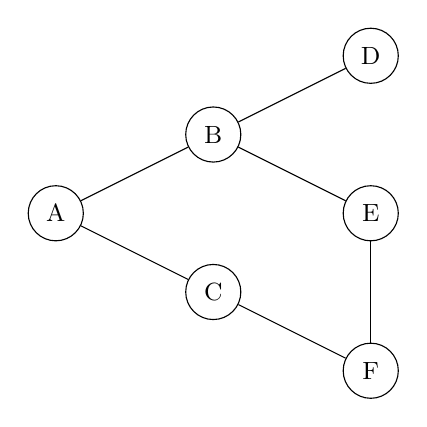
\begin{tikzpicture}[every node/.style={circle,draw,minimum size=7mm,inner sep=0pt,font=\small},scale=1]
\node (A) at (0,0) {A};
\node (B) at (2,1) {B};
\node (C) at (2,-1) {C};
\node (D) at (4,2) {D};
\node (E) at (4,0) {E};
\node (F) at (4,-2) {F};
\draw (A)--(B); \draw (A)--(C); \draw (B)--(D); \draw (B)--(E); \draw (C)--(F); \draw (E)--(F);
\end{tikzpicture}
\end{center}
\begin{lstlisting}
from collections import deque
G = {'A':['B','C'], 'B':['A','D','E'], 'C':['A','F'],
     'D':['B'],     'E':['B','F'],     'F':['C','E']}
def bfs(s):
    seen = {s}; order = []; dist = {s:0}; dq = deque([s])
    while dq:
        u = dq.popleft(); order.append(u)
        for v in G[u]:
            if v not in seen:
                seen.add(v); dist[v] = dist[u] + 1; dq.append(v)
    return order, dist
print(bfs('A'))
\end{lstlisting}
\begin{lstlisting}[style=out]
(['A', 'B', 'C', 'D', 'E', 'F'], {'A': 0, 'B': 1, 'C': 1, 'D': 2, 'E': 2, 'F': 2})
\end{lstlisting}
\begin{formula}[BFS facts]
\begin{itemize}[noitemsep]
\item Time $\Theta(V+E)$ with adjacency lists ($\Theta(V^2)$ with a matrix). Space $\Theta(V)$.
\item Gives shortest paths in \textbf{unweighted} graphs. Also used for connected components, testing bipartiteness, level-order tree traversal.
\item The BFS order depends on the order neighbours are listed in: always check the question's convention (usually alphabetical or numeric order).
\end{itemize}
\end{formula}

\subsection{Depth-first search (DFS)}
\begin{story}[Exploring a maze]
Ramu is in a maze with chalk. He walks down a corridor as far as he can; at a dead end he returns to the last junction with an unexplored path (\textbf{backtracking}) and tries that. DFS is just that: go deep first, then back up. It uses a \textbf{stack} (or recursion).
\end{story}
\begin{lstlisting}
def dfs(u, seen, order):
    seen.add(u); order.append(u)
    for v in G[u]:
        if v not in seen:
            dfs(v, seen, order)
    return order
print(dfs('A', set(), []))
\end{lstlisting}
\begin{lstlisting}[style=out]
['A', 'B', 'D', 'E', 'F', 'C']
\end{lstlisting}
Read the order: from $A$ go to $B$; from $B$ go to $D$ (dead end, back to $B$); then $E$; from $E$ go to $F$; from $F$ go to $C$. Compare with BFS on the same graph: $A,B,C,D,E,F$.
\begin{formula}[DFS facts]
\begin{itemize}[noitemsep]
\item Time $\Theta(V+E)$ with adjacency lists. Space $\Theta(V)$ (recursion depth up to $V$).
\item Each vertex gets a discovery time $d[v]$ and finish time $f[v]$. Edge types in a directed graph: \textbf{tree, back, forward, cross}. In an undirected graph only tree and back edges exist.
\item \textbf{Cycle detection:} directed graph has a cycle $\iff$ DFS finds a back edge. Undirected: an edge to an already visited vertex that is not the parent.
\item \textbf{Topological sort} (DAGs): vertices in decreasing finish time of DFS; or Kahn's algorithm: repeatedly remove a vertex of in-degree $0$. $\Theta(V+E)$. The order is generally not unique.
\item \textbf{Connected components} (undirected): run DFS/BFS from each unvisited vertex: number of runs = number of components. Strongly connected components (directed): Kosaraju/Tarjan, $\Theta(V+E)$.
\end{itemize}
\end{formula}
\begin{example}[Topological sort with Kahn's algorithm]
DAG with edges $5\to2,\ 5\to0,\ 4\to0,\ 4\to1,\ 2\to3,\ 3\to1$. In-degrees: $0{:}2,\ 1{:}2,\ 2{:}1,\ 3{:}1,\ 4{:}0,\ 5{:}0$. Start with the in-degree-0 vertices $4,5$ and repeatedly remove one and decrease its neighbours' in-degrees. One valid output (verified by code) is $4,5,2,0,3,1$. Other valid orders exist, e.g.\ $5,4,2,3,1,0$.
\end{example}

\subsection{Shortest paths}
\begin{center}
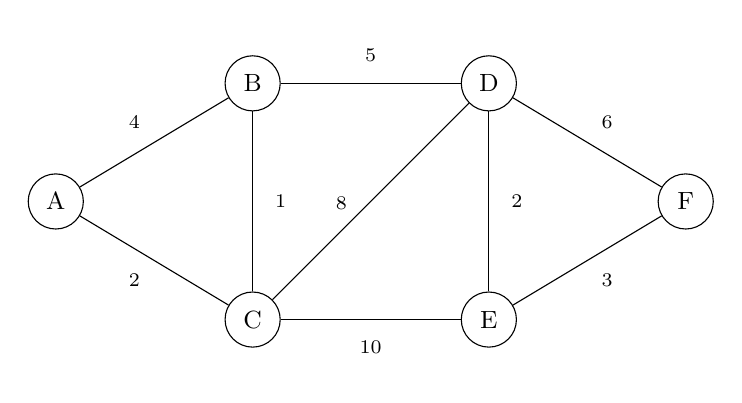
\begin{tikzpicture}[every node/.style={circle,draw,minimum size=7mm,inner sep=0pt,font=\small}]
\node (A) at (0,0) {A};
\node (B) at (2.5,1.5) {B};
\node (C) at (2.5,-1.5) {C};
\node (D) at (5.5,1.5) {D};
\node (E) at (5.5,-1.5) {E};
\node (F) at (8,0) {F};
\draw (A)--node[draw=none,above left,font=\scriptsize]{4}(B);
\draw (A)--node[draw=none,below left,font=\scriptsize]{2}(C);
\draw (B)--node[draw=none,right,font=\scriptsize]{1}(C);
\draw (B)--node[draw=none,above,font=\scriptsize]{5}(D);
\draw (C)--node[draw=none,pos=0.35,above,font=\scriptsize]{8}(D);
\draw (C)--node[draw=none,below,font=\scriptsize]{10}(E);
\draw (D)--node[draw=none,right,font=\scriptsize]{2}(E);
\draw (D)--node[draw=none,above right,font=\scriptsize]{6}(F);
\draw (E)--node[draw=none,below right,font=\scriptsize]{3}(F);
\end{tikzpicture}
\end{center}
\begin{story}[Fastest route, not fewest roads]
On Somu's map each road now has a length. The route with the fewest roads may be long in kilometres. \textbf{Dijkstra's algorithm}: keep a table of the best known distance to each village (start at $0$, others $\infty$). Repeatedly take the unfinished village with the smallest distance, and see whether going through it improves its neighbours (\textbf{relaxation}). Once a village is finished its distance is final, which is safe only because \emph{no road has negative length}.
\end{story}
\begin{lstlisting}
import heapq
W = {'A':[('B',4),('C',2)], 'B':[('A',4),('C',1),('D',5)],
     'C':[('A',2),('B',1),('D',8),('E',10)],
     'D':[('B',5),('C',8),('E',2),('F',6)],
     'E':[('C',10),('D',2),('F',3)], 'F':[('D',6),('E',3)]}
def dijkstra(s):
    dist = {v: float('inf') for v in W}; dist[s] = 0; pq = [(0, s)]
    while pq:
        d, u = heapq.heappop(pq)
        if d > dist[u]: continue                 # stale entry
        for v, w in W[u]:
            if d + w < dist[v]:                  # relaxation
                dist[v] = d + w; heapq.heappush(pq, (dist[v], v))
    return dist
print(dijkstra('A'))
\end{lstlisting}
\begin{lstlisting}[style=out]
{'A': 0, 'B': 3, 'C': 2, 'D': 8, 'E': 10, 'F': 13}
\end{lstlisting}
\begin{center}
\small
\begin{tabular}{lcccccl}
\toprule
\textbf{Step (finalise)} & \textbf{A} & \textbf{B} & \textbf{C} & \textbf{D} & \textbf{E} & \textbf{F}\\
\midrule
start & 0 & $\infty$ & $\infty$ & $\infty$ & $\infty$ & $\infty$\\
A (0) & 0 & 4 & 2 & $\infty$ & $\infty$ & $\infty$\\
C (2) & 0 & 3 & 2 & 10 & 12 & $\infty$\\
B (3) & 0 & 3 & 2 & 8 & 12 & $\infty$\\
D (8) & 0 & 3 & 2 & 8 & 10 & 14\\
E (10) & 0 & 3 & 2 & 8 & 10 & 13\\
F (13) & 0 & 3 & 2 & 8 & 10 & 13\\
\bottomrule
\end{tabular}
\end{center}
Shortest route to $F$ has length $13$: $A\to C\to B\to D\to E\to F$ ($2+1+5+2+3=13$).

\begin{formula}[Shortest path algorithms]
\begin{center}
\small
\begin{tabularx}{\textwidth}{>{\raggedright\arraybackslash}p{3.0cm} >{\raggedright\arraybackslash}p{3.8cm} >{\raggedright\arraybackslash}p{3.4cm} >{\raggedright\arraybackslash}X}
\toprule
\textbf{Algorithm} & \textbf{Solves} & \textbf{Time} & \textbf{Negative edges?}\\
\midrule
BFS & single source, unweighted & $\Theta(V+E)$ & n/a\\
Dijkstra & single source, weights $\ge0$ & $\Theta(V^2)$ array, $\Theta((V+E)\log V)$ binary heap & \textbf{no}\\
Bellman--Ford & single source & $\Theta(VE)$ & yes; detects negative cycles\\
Floyd--Warshall & all pairs & $\Theta(V^3)$ & yes (no negative cycles)\\
DAG relaxation in topological order & single source on a DAG & $\Theta(V+E)$ & yes\\
\bottomrule
\end{tabularx}
\end{center}
\textbf{Bellman--Ford:} relax \emph{all} edges, repeated $V-1$ times; one more pass that still improves something means a negative cycle is reachable. \textbf{Floyd--Warshall:} $d_{ij}\leftarrow\min(d_{ij},\,d_{ik}+d_{kj})$ for $k=1..V$ in the outer loop.
\end{formula}
\begin{example}[Bellman--Ford with a negative edge]
Edges $S\to A(4),\ S\to B(5),\ A\to C(-3),\ B\to A(-2),\ C\to D(2),\ B\to D(6)$. After $V-1=4$ rounds the distances from $S$ are $A=3$ (via $S\to B\to A$: $5-2$), $B=5$, $C=0$, $D=2$ (verified by code). Dijkstra could be fooled by edges like $-2$ because it finalises vertices too early.
\end{example}

\subsection{Bonus: minimum spanning trees}
\begin{formula}
\begin{itemize}[noitemsep]
\item A \textbf{spanning tree} of a connected graph on $n$ vertices has $n-1$ edges. The \textbf{MST} is the spanning tree of least total weight.
\item \textbf{Kruskal:} sort edges by weight, add an edge if it does not create a cycle (union--find): $\Theta(E\log E)$. \textbf{Prim:} grow a tree from a vertex, always adding the cheapest edge leaving it: $\Theta(E\log V)$ with a heap.
\item If all edge weights are distinct the MST is unique. The cheapest edge of any cut belongs to some MST.
\end{itemize}
On the weighted graph above, Kruskal picks $B$--$C$ (1), $A$--$C$ (2), $D$--$E$ (2), $E$--$F$ (3), $B$--$D$ (5) for total weight $13$. It skips $A$--$B$ (4), which would form a cycle.
\end{formula}


\subsection{DFS timestamps, edge types and graph tests}
\begin{story}[Marking time on every door]
During DFS Ramu notes a discovery time $d[v]$ when he first enters a room and a finish time $f[v]$ when he leaves it for good. Rooms entered later but left earlier are nested inside rooms entered earlier, like brackets. These timestamps classify every edge of a directed graph:
\end{story}
\begin{itemize}[noitemsep]
\item \textbf{Tree edge}: leads to an undiscovered vertex.
\item \textbf{Back edge}: leads to an ancestor still on the DFS stack. A directed graph has a cycle \emph{if and only if} DFS finds a back edge.
\item \textbf{Forward edge}: leads to a descendant already finished.
\item \textbf{Cross edge}: leads to a vertex in a different, already finished branch.
\end{itemize}
In an \emph{undirected} graph DFS only yields tree and back edges.
\begin{lstlisting}
def has_cycle_directed(g):
    color = {v: 0 for v in g}                 # 0 white, 1 grey (on stack), 2 black
    def dfs(u):
        color[u] = 1
        for w in g[u]:
            if color[w] == 1: return True     # back edge
            if color[w] == 0 and dfs(w): return True
        color[u] = 2; return False
    return any(color[v] == 0 and dfs(v) for v in g)

def bipartite(g):                              # BFS 2-colouring, g undirected
    col = {}
    for s in g:
        if s in col: continue
        col[s] = 0; q = [s]
        for u in q:
            for w in g[u]:
                if w not in col: col[w] = 1 - col[u]; q.append(w)
                elif col[w] == col[u]: return False
    return True
print(has_cycle_directed({1:[2], 2:[3], 3:[]}),
      has_cycle_directed({1:[2], 2:[3], 3:[1]}))
print(bipartite({1:[2,4], 2:[1,3], 3:[2,4], 4:[3,1]}),
      bipartite({1:[2,3], 2:[1,3], 3:[1,2]}))
\end{lstlisting}
\begin{lstlisting}[style=out]
False True
True False
\end{lstlisting}
A graph is bipartite exactly when it has \emph{no odd cycle}; the square is bipartite, the triangle is not. The number of connected components equals the number of times the outer loop starts a fresh BFS/DFS.

\subsection{Bellman--Ford, Floyd--Warshall and Prim}
\begin{story}[When roads can pay you]
Dijkstra fails if an edge has negative weight, because it assumes a finalised distance can never improve. \textbf{Bellman--Ford} makes no such assumption: it relaxes \emph{every} edge, and repeats this $V-1$ times. Any shortest path has at most $V-1$ edges, so after $V-1$ rounds all distances are correct. One more round that still improves something reveals a \textbf{negative cycle} reachable from the source.
\end{story}
\begin{lstlisting}
def bellman_ford(n, edges, s):
    d = [float('inf')]*n; d[s] = 0
    for _ in range(n-1):
        for u, v, w in edges:
            if d[u] + w < d[v]: d[v] = d[u] + w
    neg = any(d[u] + w < d[v] for u, v, w in edges)
    return d, neg
print(bellman_ford(4, [(0,1,4),(0,2,5),(1,2,-3),(2,3,2)], 0))
print(bellman_ford(3, [(0,1,1),(1,2,-1),(2,1,-1)], 0)[1])
\end{lstlisting}
\begin{lstlisting}[style=out]
([0, 4, 1, 3], False)
True
\end{lstlisting}
Time $\Theta(VE)$. In the first graph the path $0\to1\to2$ costs $4-3=1$, beating the direct edge $0\to2$ of cost $5$.

\textbf{Floyd--Warshall} computes all-pairs shortest paths by dynamic programming over ``allowed intermediate vertices'':
\[d^{(k)}_{ij}=\min\bigl(d^{(k-1)}_{ij},\ d^{(k-1)}_{ik}+d^{(k-1)}_{kj}\bigr),\]
three nested loops, time $\Theta(V^3)$, space $\Theta(V^2)$. It handles negative edges (but not negative cycles).

\textbf{Prim} grows a single tree from any start vertex, always adding the cheapest edge leaving the tree; with a binary heap it takes $\Oh(E\log V)$. Kruskal and Prim always give the same total weight (the MST weight is unique even when the tree is not).

\begin{trap}
(1) BFS/DFS visit order depends on adjacency order. (2) Dijkstra fails with negative edges; BFS gives shortest paths only when edges are unweighted. (3) A graph has a topological order iff it is a DAG. (4) $\sum\deg=2|E|$ (not $|E|$). (5) A tree on $n$ vertices has $n-1$ edges, always. (6) Adjacency matrix BFS costs $\Theta(V^2)$, not $\Theta(V+E)$.
\end{trap}

% =====================================================================

\part{Architecture Maps: Mermaid Diagrams of the Whole Subject}
\begin{story}[Maps before roads]
Ramu: ``I get lost between topics.'' Somu: ``Then look at the maps first. Each diagram below is a decision flow: it tells you \emph{what question to ask} before choosing a tool. The figures were drawn with Mermaid and the \texttt{.mmd} sources are in the companion file, so you can edit and re-render them.''
\end{story}

\section{Map 1: The whole syllabus}
\begin{center}\includegraphics[height=0.5\textheight,width=\textwidth,keepaspectratio]{d4.pdf}\end{center}

\section{Map 2: Which data structure?}
\begin{center}\includegraphics[height=0.62\textheight]{d3.pdf}\end{center}
\textbf{Reading the map.} ``Last in, first out'' means the undo button of an editor, and also the call stack of recursion: use a list with \py{append}/\py{pop}. ``First in, first out'' means a canteen queue and BFS: use \py{collections.deque}, because \py{list.pop(0)} costs $O(n)$. Fast lookup by key is the phone book: a hash table gives $O(1)$ average. Repeatedly asking for the smallest is a hospital triage desk: a heap gives $O(\log n)$.

\section{Map 3: Merge sort as divide and conquer}
\begin{center}\includegraphics[width=0.7\textwidth]{d5.pdf}\end{center}
The three words to remember are \textbf{split, solve, combine}. Merge sort's work is in the combine step ($O(n)$ per level, $\log_2 n$ levels, hence $\Theta(n\log n)$). Quicksort puts its work in the split step instead (partitioning).

\section{Map 4: BFS flow}
\begin{center}\includegraphics[height=0.55\textheight]{d6.pdf}\end{center}
The queue is the reason BFS finds \emph{fewest edges}: vertices come out in non-decreasing distance order, like ripples spreading from a stone dropped in a pond.

\section{Map 5: DFS and edge colours}
\begin{center}\includegraphics[width=0.95\textwidth]{d7.pdf}\end{center}
In an \textbf{undirected} graph DFS produces only tree and back edges. In a \textbf{directed} graph it can also produce forward and cross edges; a directed graph has a cycle iff DFS finds a back edge (GRAY neighbour).

\section{Map 6: Which Google-style pattern?}
\begin{center}\includegraphics[height=0.5\textheight,width=\textwidth,keepaspectratio]{d8.pdf}\end{center}
This map is expanded with code in Part V.

\part{Previous GATE DA Questions (2024, 2025, 2026) Solved One by One}

\begin{story}[Why read old papers?]
Ramu: ``Will the same questions come again?'' Somu: ``Not the same, but the \emph{same ideas} in new clothes. A question on quicksort pivots in 2024 becomes a recurrence question in 2026. So we solve each old question, then ask what idea it tested.''
\end{story}

\textbf{About these questions.} Statements are paraphrased from the official GATE DA papers and answer keys of 2024, 2025 and 2026 (the 2025 stems are taken from a published solutions PDF, and every answer was matched with the official key); code is restated in equivalent Python. Questions that depend on a figure not available in text are solved by \emph{method} using the facts that are stated. Every answer was also checked by running code or by brute force. Questions belonging to other sections (DBMS B+ trees, AI search) are not repeated here.

\section{2024 Programming, Data Structures and Algorithms}

\begin{example}[{2024 Q14 (1 mark, MCQ): edge type in DFS --- key A (Tree)}]
\textbf{Question.} DFS on an undirected unweighted graph from $s$; $d[u]$ is the shortest distance from $s$. An edge $(u,v)$ has $d[u]<d[v]$ and DFS first traverses it from $u$ to $v$. Tree, cross, back or gray?\\
\textbf{Idea.} Undirected DFS has only tree and back edges, so cross is impossible. A back edge goes from a vertex to its \emph{ancestor}, which was discovered earlier and normally is closer to the source. With $d[u]<d[v]$, the edge goes ``downward'', so the intended answer is \textbf{Tree} (A). ``Gray'' is a vertex colour, not an edge type.\\
\textbf{Honest note.} Under a fully literal reading I found, by brute force, a graph where this breaks: edges $\{0\!-\!1,0\!-\!2,1\!-\!3,1\!-\!4,2\!-\!3,3\!-\!4\}$ with DFS visiting neighbours in descending order reaches vertex 1 \emph{after} 3 and 4, so $(1,3)$ is a back edge although $d[1]=1<d[3]=2$. The official key still says A; choose A in the exam and remember the intended logic: \emph{downward in distance means tree}.
\end{example}

\begin{example}[{2024 Q16 (1 mark, MCQ): match structure to behaviour --- key A}]
FIFO $\to$ queues, lookup $\to$ hash tables, LIFO $\to$ stacks: option A (p--ii, q--iii, r--i). \textbf{Connect:} Map 2.
\end{example}

\begin{example}[{2024 Q21 (1 mark, MCQ): open addressing --- key B}]
With uniform hashing and load factor $\alpha=n/m<1$, the expected number of probes for an \emph{unsuccessful} search is at most $\frac1{1-\alpha}$, and the same bound holds for an insertion (an insertion first fails to find an empty slot, then uses one). Answer: $\frac1{1-\alpha}$.\\
\textbf{Why.} Each probe hits an occupied slot with probability about $\alpha$, so the number of probes is geometric: $1+\alpha+\alpha^2+\dots=\frac1{1-\alpha}$. At $\alpha=0.5$ that is 2 probes; at $\alpha=0.9$ it is 10, which is why real tables resize before getting full.
\end{example}

\begin{example}[{2024 Q28 (1 mark, MSQ): which traversal pairs rebuild a \emph{full} binary tree --- key A, B, C}]
In a \emph{full} binary tree every node has 0 or 2 children. Then preorder+inorder, inorder+postorder \emph{and} preorder+postorder each give a unique tree. (For general binary trees, preorder+postorder is ambiguous when a node has a single child, because you cannot tell left from right; fullness removes that ambiguity.) \textbf{Trap:} option D (inorder alone) never suffices.
\end{example}

\begin{example}[{2024 Q30 (1 mark, NAT): quicksort swaps on sorted data --- key 0}]
Array $60,70,80,90,100$, in-place quicksort with the last element as pivot. Minimum number of swaps?\\
Partition scans $j$ from left; every element is $\le$ pivot $100$, so $i$ moves in step with $j$ and each ``swap'' exchanges an element with itself (no real change). The pivot also lands in its own place. So the number of \emph{real} swaps is $\mathbf{0}$; this is the same input that is the \emph{worst case} for time ($\Theta(n^2)$ comparisons, recursion depth $n$) but needs no actual movement. I verified by running quicksort with a ``swap only if $i\ne j$'' guard.\\
\textbf{Lesson.} Number of comparisons, swaps and time are three different quantities.
\end{example}

\begin{example}[{2024 Q32 (1 mark, NAT): deque simulation --- key 17}]
Track the deque (front on the left):
\begin{center}
\begin{tabular}{llc}\toprule
step & operation & deque\\\midrule
1 & insertFirst(10) & [10]\\
2 & insertLast(32) & [10, 32]\\
3 & a $\gets$ removeFirst() (10) & [32]\\
4 & insertLast(28) & [32, 28]\\
5 & insertLast(17) & [32, 28, 17]\\
6 & a $\gets$ removeFirst() (32) & [28, 17]\\
7 & a $\gets$ removeLast() & [28]\\\bottomrule
\end{tabular}
\end{center}
Step 7 returns \textbf{17}, so $a=17$. Habit: draw the container after every line.
\end{example}

\begin{example}[{2024 Q38 (1 mark, MCQ): recursion on a tree stored in a dict --- key D (9)}]
\py{count(tree,node)} returns $1+\sum$ of its children's counts, and returns $1$ for a node with no entry in the dict (a leaf). The dictionary describes root $0$ with children $1,2$; node $1$ has $3,4,5$; node $2$ has $6,7,8$. Each of the six grandchildren $3..8$ is a leaf (count 1); node $1$ gives $1+3=4$, node $2$ gives $1+3=4$, so the root gives $1+4+4=\mathbf 9$ (the \emph{number of nodes}). Output: 9.
\end{example}

\begin{example}[{2024 Q39 (1 mark, MCQ): the ``stock span'' style array --- key C}]
$S[i]$ starts at $1$ and becomes $1+S[i-1]$ when $X[i-1]\le X[i]$.\\
$X=[6,3,5,4,10]$: $S_0=1$; $3\ge6$? no $\Rightarrow1$; $5\ge3$ yes $\Rightarrow1+1=2$; $4\ge5$? no $\Rightarrow1$; $10\ge4$ yes $\Rightarrow1+1=2$. Answer $[1,1,2,1,2]$ (C). It is the length of the longest non-decreasing run ending at $i$: options A and D count values that would require chains the code never builds.
\end{example}

\begin{example}[{2024 Q40 (1 mark, MCQ): recurrence of binary search --- key A}]
One comparison with the middle element, then recurse into one half of size at most $\lfloor n/2\rfloor$: $F(n)=F(\lfloor n/2\rfloor)+1$. Option B would describe doing \emph{both} halves (merge-sort-like).
\end{example}

\begin{example}[{2024 Q41 (1 mark, MCQ): what does \py{fun} do --- key C (reverse)}]
\begin{lstlisting}
def fun(D,s1,s2):
    if s1<s2:
        D[s1],D[s2]=D[s2],D[s1]
        fun(D,s1+1,s2-1)
\end{lstlisting}
It swaps the two ends, then moves both ends inward: that is reversing \py{D[s1..s2]}. Test: \py{[1,2,3,4,5]} with $(0,4)$ becomes \py{[5,4,3,2,1]}; \py{[1,2,3,4,5,6]} with $(1,4)$ becomes \py{[1,5,4,3,2,6]}. This is the two-pointer pattern of Part V.
\end{example}

\begin{example}[{2024 Q44 (1 mark, MCQ): BFS versus DFS on a number graph --- key C (same number)}]
States $n\to n+1,n+2$, expanded in ascending order, goal $6$. BFS expands $1,2,3,4,5,6$ (six states) level by level. The key says DFS also expands six states under the question's tie rule, so both expand the same number of states. \textbf{Lesson:} counts depend on the stated rule for tie-breaking and re-adding; read that rule before computing.
\end{example}

\begin{example}[{2024 Q45 (1 mark, MCQ): sorted after exactly two passes? --- key B (selection only)}]
Start $[4,3,2,1,5]$.
\begin{center}
\begin{tabular}{lll}\toprule
Algorithm & after pass 1 & after pass 2\\\midrule
Bubble & $[3,2,1,4,5]$ & $[2,1,3,4,5]$\\
Insertion & $[3,4,2,1,5]$ & $[2,3,4,1,5]$\\
Selection & $[1,3,2,4,5]$ & $[1,2,3,4,5]$ \checkmark\\\bottomrule
\end{tabular}
\end{center}
Only selection sort is fully sorted, because after two passes it has placed the two smallest elements and the rest was already in order.
\end{example}

\begin{example}[{2024 Q51 (MSQ, figure-based): valid topological orders --- key B, D}]
The DAG figure is not available in text, so I only give the method: an ordering is valid iff every edge $u\to v$ has $u$ before $v$. Check each option against \emph{every} edge, or run Kahn's algorithm (Part V) and see which orderings it can produce. (My inference, not from the paper: options A and C both put $Q$ before $R$ while B and D put $R$ before $Q$, which suggests the figure has an edge $R\to Q$.)
\end{example}

\begin{example}[{2024 Q52 (MSQ): facts about binary trees --- key A, B, C}]
$H$ = height (edges on longest path), $I$ internal, $L$ leaves, $N$ nodes.
\begin{itemize}[leftmargin=*,itemsep=1pt]
\item \textbf{(A) $L\le I+1$ true}: nodes with 2 children $+1$ equals leaves; nodes with one child only add to $I$.
\item \textbf{(B) $H+1\le N\le2^{H+1}-1$ true}: at least a path of $H+1$ nodes, at most a perfect tree.
\item \textbf{(C) $H\le I\le2^H-1$ true}: the longest path has $H$ internal nodes; a perfect tree has $2^H-1$.
\item \textbf{(D) $H\le L\le2^{H-1}$ false}: perfect tree of height $H$ has $2^H$ leaves; a tree of height 1 has up to 2 leaves but the bound gives $1$.
\end{itemize}
I brute-forced all binary tree shapes up to $9$ nodes and confirmed A, B, C always hold and D fails.
\end{example}

\section{2025 Programming, Data Structures and Algorithms}

\begin{example}[{2025 Q18 (1 mark, MCQ): hashing with linear probing --- key D (4 and 6)}]
$h(x)=3x\bmod10$, table size 10, insert $1,4,5,6,14,15$.
\begin{center}
\begin{tabular}{cccl}\toprule
key & $h$ & probes & lands at\\\midrule
1 & 3 & 3 free & 3\\
4 & 2 & 2 free & 2\\
5 & 5 & 5 free & 5\\
6 & 8 & 8 free & 8\\
14 & 2 & 2 busy, 3 busy, 4 free & \textbf{4}\\
15 & 5 & 5 busy, 6 free & \textbf{6}\\\bottomrule
\end{tabular}
\end{center}
Final table: index 2:4, 3:1, 4:14, 5:5, 6:15, 8:6. Answer: 14 at 4, 15 at 6.
\end{example}

\begin{example}[{2025 Q23 and Q27 (1 mark each, MCQ)}]
\textbf{Q23 key A:} \py{A.extend(B)} appends the items of $B$ one by one, giving \py{[1,2,3,4,5,6]}; \py{append(B)} would nest the list, and \py{update}/\py{insert(B)} do not do this. \textbf{Q27 key C:} binary search needs random access and sorted order, so an increasing \emph{array}; a linked list cannot jump to the middle in $O(1)$.
\end{example}

\begin{example}[{2025 Q29 (1 mark, MSQ): insertion sort with exactly two swaps --- key A, C}]
Array $[1,3,5,7,9,11,x,15,13]$. The number of swaps in insertion sort equals the number of \emph{inversions} (pairs out of order). The pair $(15,13)$ is always one inversion, so $x$ must create exactly one more.
\begin{center}
\begin{tabular}{cl c}\toprule
$x$ & elements before $x$ larger than $x$, and elements after smaller than $x$ & total\\\midrule
10 & before: $11$ ($1$); after: none ($15,13>10$) & $1+1=2$ \checkmark\\
12 & before: none; after: none & $0+1=1$\\
14 & before: none; after: $13$ ($1$) & $1+1=2$ \checkmark\\
16 & before: none; after: $15,13$ ($2$) & $2+1=3$\\\bottomrule
\end{tabular}
\end{center}
\textbf{Lesson:} swaps in insertion sort = inversions; count inversions instead of simulating.
\end{example}

\begin{example}[{2025 Q47 (2 marks, MCQ): set operations in a loop --- key B (only B)}]
Start $A=\{\text{this,that}\}$, $B=\{\text{that,other}\}$, $C=\{\text{other,this}\}$; loop while ``other'' $\in C$. Python evaluates the right side before assigning, so the three updates use the \emph{old} values together.\\
\textbf{Iteration 1.} ``this'' $\in A$, so $A,B,C\gets A\!-\!B,\ B\!-\!C,\ C\!-\!A=\{\text{this}\},\{\text{that}\},\{\text{other}\}$.\\
Then ``that'' $\in B$: $A,B,C\gets C|A,\ A|B,\ B|C=\{\text{other,this}\},\{\text{this,that}\},\{\text{that,other}\}$.\\
\textbf{Iteration 2.} ``other'' $\in C$ still: ``this'' $\in A$: $A-B=\{\text{other}\}$, $B-C=\{\text{this}\}$, $C-A=\{\text{that}\}$ so $A=\{\text{other}\}$, $B=\{\text{this}\}$, $C=\{\text{that}\}$. ``that'' $\in B$? No. Loop test: ``other'' $\in C$? No: stop.\\
Only $B$ contains ``this''. (I ran this program and obtained exactly these sets.)
\end{example}

\begin{example}[{2025 Q58 (2 marks, MSQ, figure-based): which pairs are NOT edges --- key A, C, D}]
Facts stated: $a\!-\!b\!-\!c\!-\!d$ is a shortest path $a\to d$; $e\!-\!f\!-\!g\!-\!h$ is a shortest path $e\to h$; $a\!-\!f\!-\!c\!-\!h$ is a shortest path $a\to h$. A sub-path of a shortest path is itself shortest, so:
\begin{itemize}[leftmargin=*,itemsep=1pt]
\item $d(b,d)=2$, so $(b,d)$ is not an edge $\Rightarrow$ A is a non-edge.
\item $d(a,h)=3$. An edge $(b,h)$ would give $a\!-\!b\!-\!h$ of length 2, contradiction $\Rightarrow$ C is a non-edge.
\item $d(e,g)=2$ (sub-path of $e\!-\!f\!-\!g\!-\!h$), so $(e,g)$ is not an edge $\Rightarrow$ D is a non-edge.
\item $(b,g)$: $a\!-\!b\!-\!g\!-\!h$ has length 3, no contradiction, so it \emph{may} be an edge; B is not forced.
\end{itemize}
Answer A, C, D. I derived this from the stated facts alone, without needing the figure.
\end{example}

\begin{example}[{2025 Q63 (2 marks, NAT): a recursion that only takes the odd branch --- key 160}]
\begin{lstlisting}
def f(a,b):
    if a==0: return b
    if a%2==1: return 2*f((a-1)//2,b)
    return b+f((a-1)//2,b)
print(f(15,10))
\end{lstlisting}
(The printed source text is garbled; the version above is the reading that reproduces the official key $160$.) $a$ goes $15\to7\to3\to1\to0$, always odd, so the even branch never runs: $f(15)=2f(7)=4f(3)=8f(1)=16f(0)=16\cdot10=\mathbf{160}$. Each odd step doubles the answer: four doublings of $b=10$.
\end{example}

\begin{example}[{2025 Q64 (2 marks, NAT): stack simulation --- key 24}]
Push $0$. The loop pushes $1,2,\dots,8$ until $x=8$ sets \py{flag=1}; from then on each round pops $x$, pops one more if $x$ is odd, and adds $x$ to the sum.
\begin{center}
\begin{tabular}{llcl}\toprule
round & stack before popping & pop $x$ & extra pop; sum\\\midrule
1 & $0..8$ & 8 & none; $8$\\
2 & $0..7$ & 7 odd & pop 6; $15$\\
3 & $0..5$ & 5 odd & pop 4; $20$\\
4 & $0..3$ & 3 odd & pop 2; $23$\\
5 & $0,1$ & 1 odd & pop 0; $24$\\\bottomrule
\end{tabular}
\end{center}
Stack empty; output $\mathbf{24}$. Check: $8+7+5+3+1=24$.
\end{example}

\begin{example}[{2025 Q65 (2 marks, NAT): DFS on a staircase graph --- key 75}]
Vertices $0..100$, edges $i\to j$ if $1\le j-i\le2$, neighbours tried in \emph{decreasing} order, so from $i$ DFS tries $i+2$ before $i+1$. From $0$: $0,2,4,\dots,100$ (all evens, 51 vertices). Vertex $100$ has no outgoing edge, so DFS backs up to $98$, which tries $99$, then to $96$, which tries $97$, and so on: odd vertices are discovered in order $99,97,\dots,1$. Vertex $50$ is the 26th discovered, so $101-26=\mathbf{75}$ vertices are discovered after it (the 25 evens $52..100$ and the 50 odds).
\end{example}

\section{2026 Programming, Data Structures and Algorithms}

\begin{example}[{2026 Q15 (1 mark, MCQ): expected time of quicksort --- key D}]
With the first element as pivot and \emph{random} order, the pivot's rank is uniform, so $T(n)=\frac1n\sum_{k=0}^{n-1}\big[T(k)+T(n-k-1)\big]+O(n)$ (D). Option A is the worst case (pivot always extreme), B is a lucky fixed split, C is the best case. Solving D gives $\Theta(n\log n)$. \textbf{Connect:} 2024 Q30 was the worst-case input.
\end{example}

\begin{example}[{2026 Q16 (1 mark, MCQ): the shared default list --- key B}]
\begin{lstlisting}
def append_to_lst(val, lst=[]):
    lst.append(val); return lst
print(append_to_lst(1)); print(append_to_lst(2)); print(append_to_lst(3, []))
\end{lstlisting}
\begin{lstlisting}[style=out]
[1]
[1, 2]
[3]
\end{lstlisting}
The default \py{[]} is created \emph{once} when the \py{def} runs and is reused by every call that omits \py{lst}. The third call passes a fresh list. Safe pattern: \py{lst=None} and \py{if lst is None: lst=[]}.
\end{example}

\begin{example}[{2026 Q25 (1 mark, MSQ): rebuild a tree from two traversals --- key A, B}]
Preorder $P\,Q\,S\,E\,R\,F\,G$, inorder $S\,Q\,E\,P\,F\,R\,G$. Preorder's first letter is the root: $P$ (A true). In inorder, left of $P$ is $\{S,Q,E\}$ and right is $\{F,R,G\}$. Left subtree: preorder $Q\,S\,E$, root $Q$, inorder $S\,Q\,E$ so $S$ left, $E$ right. Right subtree: preorder $R\,F\,G$, root $R$ with $F$ left and $G$ right.
\begin{center}
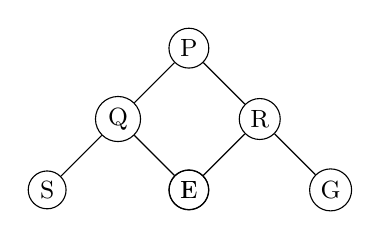
\begin{tikzpicture}[level distance=9mm,sibling distance=18mm,every node/.style={circle,draw,inner sep=2pt,font=\small}]
\node{P} child{node{Q} child{node{S}} child{node{E}}} child{node{R} child{node{F}} child{node{G}}};
\end{tikzpicture}
\end{center}
Postorder (left, right, root): $S\,E\,Q\,F\,G\,R\,P$ (B true). $Q$ has two children (C false). The left subtree of $R$ is $F$, not $G$ (D false).
\end{example}

\begin{example}[{2026 Q31 (1 mark, NAT): binary search comparisons when absent --- key 10}]
Sorted array of $n=1000$ distinct integers; each step compares the middle element with $y$ (equal / less / greater counts as \emph{one} comparison). The worst number of steps is the number of times you can halve until empty: $\lfloor\log_2 n\rfloor+1=\lfloor9.97\rfloor+1=\mathbf{10}$. Check: after 9 halvings up to $1000/2^9\approx1.95$ elements remain, so a 10th look is needed. (If two comparisons were counted per step, the answer would be 20; read the question's counting rule.)
\end{example}

\begin{example}[{2026 Q39 (2 marks, MCQ): counting recursive calls --- key C (15)}]
$\text{mystery}(n)$ returns 1 for $n\le0$, else $\text{mystery}(n-1)+\text{mystery}(n-2)$. Let $C(n)$ be the number of calls: $C(n)=1+C(n-1)+C(n-2)$ with $C(0)=C(-1)=1$ (and every $n\le0$ is a single call).
\begin{center}
\begin{tabular}{c|cccccc}$n$&$-1$&$0$&$1$&$2$&$3$&$4$\\\hline $C(n)$&1&1&$1+1+1=3$&$1+3+1=5$&$1+5+3=9$&$1+9+5=\mathbf{15}$\end{tabular}
\end{center}
Answer 15 (I confirmed it with a call counter). \textbf{Lesson:} such counts grow like Fibonacci, exponentially; memoisation (Part V) cuts it to linear.
\end{example}

\begin{example}[{2026 Q40 (2 marks, MCQ): reverse graph reachability --- key D}]
$G^R$ has every edge reversed. A path $v\to\dots\to u$ in $G$ becomes a path $u\to\dots\to v$ in $G^R$. So if DFS from $v$ in $G$ reaches $u$, then BFS from $u$ in $G^R$ reaches $v$: option D. Option A reverses the direction (it would need $u\to v$ in $G$). Options B and C claim equal visited sets or reversed orders, which are false in general because $G^R$ explores different paths.
\end{example}

\begin{example}[{2026 Q49 (2 marks, MSQ): bubble sort versus insertion sort on $[1,2,3,5,4]$ --- key B, C, D}]
Bubble sort (no early stopping) makes $4+3+2+1=10$ comparisons ($N_1=10$). Insertion sort compares: $(1,2)$, $(2,3)$, $(3,5)$, then $5$ vs $4$ (swap) and $3$ vs $4$ (stop): $N_2=5$.
\begin{itemize}[leftmargin=*,itemsep=1pt]
\item (A) $N_1=10$ but $N_2=5\ne4$: false.
\item (B) $N_1>N_2$: $10>5$ true.
\item (C) insertion sort does exactly one swap ($5,4$): true.
\item (D) both compare pairs that were already in order, such as $(1,2)$: true.
\end{itemize}
Bubble sort with an early-exit flag would stop after the second pass ($7$ comparisons) but the question counts the plain version.
\end{example}

\begin{example}[{2026 Q50 (2 marks, MSQ): closures keep their own list --- key B, D}]
Each call of \py{outer()} creates a \emph{new} list \py{x} captured by its own \py{inner}. So \py{f1} and \py{f2} do \emph{not} share (A false). \py{f1(10)}$\to[10]$, \py{f1(20)}$\to[10,20]$ (B true), \py{f2(30)}$\to[30]$ (C false), \py{f1(40)}$\to[10,20,40]$ (D true; \py{f2} never touched \py{f1}'s list).
\end{example}

\begin{example}[{2026 Q58 (2 marks, NAT): a recursive bubble pass --- key 8}]
\py{fun(L)} walks left to right, swapping each out-of-order neighbour pair and counting swaps: one bubble pass. It is called $5$ times on $[5,3,4,1,2]$.
\begin{center}
\begin{tabular}{cccl}\toprule
pass & swaps & list afterwards & running total\\\midrule
1 & 4 & $[3,4,1,2,5]$ & 4\\
2 & 2 & $[3,1,2,4,5]$ & 6\\
3 & 2 & $[1,2,3,4,5]$ & 8\\
4--5 & 0 & sorted & 8\\\bottomrule
\end{tabular}
\end{center}
Output $\mathbf{8}$. Why this must equal the number of \emph{inversions} of $[5,3,4,1,2]$: each adjacent swap removes exactly one inversion, and inversions are $(5,3),(5,4),(5,1),(5,2),(3,1),(3,2),(4,1),(4,2)=8$.
\end{example}

\section{Ideas the Questions Tested (the real syllabus)}
\begin{center}\small
\begin{tabularx}{\textwidth}{lX}\toprule
Idea & Appears in\\\midrule
Trace and simulate (tables) & 2024 Q32, Q39, 2025 Q18, Q64, 2026 Q58\\
Recursion on trees / counts & 2024 Q38, 2025 Q63, 2026 Q39\\
Mutable state, aliasing, closures & 2026 Q16, Q50, 2025 Q23, Q47\\
Sorting passes, swaps, comparisons & 2024 Q30, Q45, 2025 Q29, 2026 Q15, Q49, Q58\\
Inversions = adjacent swaps & 2025 Q29, 2026 Q58\\
Binary search and halving & 2024 Q40, 2025 Q27, 2026 Q31\\
Traversals and tree shape & 2024 Q28, Q52, 2026 Q25\\
Graph search facts & 2024 Q14, Q44, Q51, 2025 Q58, Q65, 2026 Q40\\
Hashing & 2024 Q21, 2025 Q18\\\bottomrule
\end{tabularx}
\end{center}
\textbf{Pattern:} 1-mark questions test one rule exactly; 2-mark questions chain a trace with a property (count, inversions, pass behaviour). Practise tracing by hand with a table.

\part{Google-style Interview Preparation}

\begin{story}[Same tools, sharper habits]
Ramu: ``Is Google prep different from GATE?'' Somu: ``GATE gives you the code and asks the output. An interview gives you a sentence and asks you to \emph{invent} the code. The tools (arrays, hash maps, heaps, BFS, binary search) are the same. What changes is that you must (1) clarify the problem, (2) pick a pattern, (3) code it cleanly, (4) test edge cases, (5) state the complexity. Practise this five-step routine out loud.''
\end{story}

\section{The Five-Step Routine}
\begin{enumerate}[leftmargin=*,itemsep=2pt]
\item \textbf{Clarify:} input size, duplicates, negatives, sorted or not, empty input, what to return when nothing is found.
\item \textbf{Brute force first:} state the obvious $O(n^2)$ or exponential solution and its cost. This shows you understand the problem and gives you a baseline to improve.
\item \textbf{Find the waste:} which work is repeated? Repeated lookups suggest a hash map; repeated range sums suggest prefix sums; repeated sorting-like scans suggest a heap or binary search.
\item \textbf{Code} with meaningful names; \textbf{test} on a tiny example and on edge cases ($n=0,1$, all equal, negative values).
\item \textbf{State time and space complexity} and what you would improve with more time.
\end{enumerate}

\section{Pattern 1: Hash Map (``have I seen the partner?'')}
\textbf{Two Sum:} find indices of two numbers adding to a target. Brute force checks every pair, $O(n^2)$. Waste: for each $x$ we search the whole array for $t-x$. Fix: store seen values in a dict, so each lookup is $O(1)$.
\begin{lstlisting}
def two_sum(a,t):
    seen={}
    for i,x in enumerate(a):
        if t-x in seen: return (seen[t-x],i)
        seen[x]=i
print(two_sum([2,7,11,15],9))
\end{lstlisting}
\begin{lstlisting}[style=out]
(0, 1)
\end{lstlisting}
Time $O(n)$, space $O(n)$. \textbf{Why correct:} when we reach the second element of the pair, the first is already in the dict.

\section{Pattern 2: Two Pointers (sorted data)}
\begin{lstlisting}
def two_ptr(a,t):                 # a is sorted
    i,j=0,len(a)-1
    while i<j:
        s=a[i]+a[j]
        if s==t: return (i,j)
        i,j=(i+1,j) if s<t else (i,j-1)
print(two_ptr([1,3,4,6,9],10))
\end{lstlisting}
\begin{lstlisting}[style=out]
(0, 4)
\end{lstlisting}
If the sum is too small, the smallest element can never work with anything smaller than the current right end, so discard it; symmetric for too large. $O(n)$ time, $O(1)$ space. The reversal in 2024 Q41 is the same two-pointer walk.

\section{Pattern 3: Sliding Window}
Best sum of $k$ consecutive items: instead of re-adding $k$ numbers each time, add the new element and subtract the one that left.
\begin{lstlisting}
def best_window(a,k):
    s=sum(a[:k]); b=s
    for i in range(k,len(a)):
        s+=a[i]-a[i-k]; b=max(b,s)
    return b
print(best_window([2,1,5,1,3,2],3))
\end{lstlisting}
\begin{lstlisting}[style=out]
9
\end{lstlisting}
Variable-size window, \textbf{longest substring without repeats}: keep the window start \py{l}, jump it past the previous occurrence of the current character.
\begin{lstlisting}
def longest_unique(s):
    last={}; l=0; b=0
    for r,ch in enumerate(s):
        if ch in last and last[ch]>=l: l=last[ch]+1
        last[ch]=r; b=max(b,r-l+1)
    return b
print(longest_unique("abcabcbb"))
\end{lstlisting}
\begin{lstlisting}[style=out]
3
\end{lstlisting}

\section{Pattern 4: Prefix Sums}
Let $P[i]$ be the sum of the first $i$ items. Then the sum of items $i..j-1$ is $P[j]-P[i]$, answered in $O(1)$ after $O(n)$ preparation.
\begin{lstlisting}
P=[0]
for x in [3,1,4,1,5,9]: P.append(P[-1]+x)
print(P, P[5]-P[2])
\end{lstlisting}
\begin{lstlisting}[style=out]
[0, 3, 4, 8, 9, 14, 23] 10
\end{lstlisting}
Here $P[5]-P[2]=14-4=10=4+1+5$. Rule of thumb: many range-sum queries means prefix sums.

\section{Pattern 5: Binary Search on the Answer}
Binary search is not only for arrays. If you can write a yes/no test \py{ok(x)} that is \emph{monotone} (false\dots false true\dots true), you can binary-search $x$. Example (``Koko eating bananas''): smallest speed $k$ so that piles $[3,6,7,11]$ are finished within $8$ hours, where each hour eats from one pile at most $k$.
\begin{lstlisting}
def min_speed(piles,h):
    lo,hi=1,max(piles)
    while lo<hi:
        m=(lo+hi)//2
        if sum(-(-p//m) for p in piles)<=h: hi=m
        else: lo=m+1
    return lo
print(min_speed([3,6,7,11],8))
\end{lstlisting}
\begin{lstlisting}[style=out]
4
\end{lstlisting}
\py{-(-p//m)} is ceiling division. Complexity $O(n\log\max)$. Counting steps of plain binary search (as in 2026 Q31):
\begin{lstlisting}
def binsearch(a,t):
    lo,hi=0,len(a)-1; c=0
    while lo<=hi:
        c+=1; m=(lo+hi)//2
        if a[m]==t: return m,c
        if a[m]<t: lo=m+1
        else: hi=m-1
    return -1,c
print(binsearch([1,3,5,7,9,11,13],11), binsearch(list(range(1000)),999))
\end{lstlisting}
\begin{lstlisting}[style=out]
(5, 2) (999, 10)
\end{lstlisting}

\section{Pattern 6: Stack and Monotonic Stack}
\textbf{Balanced brackets} use a stack: push openers, and every closer must match the top.
\begin{lstlisting}
def valid(s):
    st=[]; m={')':'(',']':'[','}':'{'}
    for ch in s:
        if ch in m:
            if not st or st.pop()!=m[ch]: return False
        else: st.append(ch)
    return not st
print(valid("{[()]}"), valid("([)]"))
\end{lstlisting}
\begin{lstlisting}[style=out]
True False
\end{lstlisting}
\textbf{Next greater element:} keep a stack of indices whose answer is still unknown, with decreasing values; a bigger new value answers all smaller ones on top. Each index is pushed and popped once, so $O(n)$ even though there is a loop inside a loop.
\begin{lstlisting}
def next_greater(a):
    r=[-1]*len(a); st=[]
    for i,x in enumerate(a):
        while st and a[st[-1]]<x: r[st.pop()]=x
        st.append(i)
    return r
print(next_greater([2,1,2,4,3]))
\end{lstlisting}
\begin{lstlisting}[style=out]
[4, 2, 4, -1, -1]
\end{lstlisting}

\section{Pattern 7: Heap (top-$k$)}
Keep a min-heap of size $k$; the root is the smallest of the current top $k$. Each push/pop is $O(\log k)$, so total $O(n\log k)$ rather than sorting in $O(n\log n)$.
\begin{lstlisting}
import heapq
def topk(a,k):
    h=[]
    for x in a:
        heapq.heappush(h,x)
        if len(h)>k: heapq.heappop(h)
    return sorted(h,reverse=True)
print(topk([5,1,9,3,7,8],3))
\end{lstlisting}
\begin{lstlisting}[style=out]
[9, 8, 7]
\end{lstlisting}

\section{Pattern 8: BFS/DFS on a Grid}
\textbf{Count islands:} each unvisited land cell starts a new island; BFS marks the whole island. Total $O(RC)$.
\begin{lstlisting}
from collections import deque
def islands(g):
    R,C=len(g),len(g[0]); seen=set(); n=0
    for r in range(R):
        for c in range(C):
            if g[r][c]==1 and (r,c) not in seen:
                n+=1; q=deque([(r,c)]); seen.add((r,c))
                while q:
                    y,x=q.popleft()
                    for dy,dx in ((1,0),(-1,0),(0,1),(0,-1)):
                        ny,nx=y+dy,x+dx
                        if 0<=ny<R and 0<=nx<C and g[ny][nx]==1 and (ny,nx) not in seen:
                            seen.add((ny,nx)); q.append((ny,nx))
    return n
print(islands([[1,1,0,0],[0,1,0,1],[1,0,0,1]]))
\end{lstlisting}
\begin{lstlisting}[style=out]
3
\end{lstlisting}
\textbf{Topological sort (Kahn):} repeatedly remove a vertex with in-degree 0. If fewer than $n$ vertices are removed, there is a cycle.
\begin{lstlisting}
def topo(n,edges):
    adj=[[] for _ in range(n)]; ind=[0]*n
    for u,v in edges: adj[u].append(v); ind[v]+=1
    q=deque(i for i in range(n) if ind[i]==0); o=[]
    while q:
        u=q.popleft(); o.append(u)
        for v in adj[u]:
            ind[v]-=1
            if ind[v]==0: q.append(v)
    return o if len(o)==n else None
print(topo(6,[(5,2),(5,0),(4,0),(4,1),(2,3),(3,1)]), topo(3,[(0,1),(1,2),(2,0)]))
\end{lstlisting}
\begin{lstlisting}[style=out]
[4, 5, 2, 0, 3, 1] None
\end{lstlisting}

\section{Pattern 9: Dynamic Programming in Two Lines of Thought}
\textbf{Memoisation} stores answers of repeated sub-calls; the exponential recursion of 2026 Q39 becomes linear.
\begin{lstlisting}
def fib_memo():
    memo={}
    def f(n):
        if n<2: return n
        if n not in memo: memo[n]=f(n-1)+f(n-2)
        return memo[n]
    return f
print(fib_memo()(50))
\end{lstlisting}
\begin{lstlisting}[style=out]
12586269025
\end{lstlisting}
\textbf{Kadane (maximum subarray):} the best sum ending here is either the element alone or it extended by the best sum ending at the previous place.
\begin{lstlisting}
def kadane(a):
    cur=best=a[0]
    for x in a[1:]:
        cur=max(x,cur+x); best=max(best,cur)
    return best
print(kadane([-2,1,-3,4,-1,2,1,-5,4]))
\end{lstlisting}
\begin{lstlisting}[style=out]
6
\end{lstlisting}
The winning window is $[4,-1,2,1]$ with sum $6$.

\section{Divide and Conquer, Once More with Code}
\begin{lstlisting}
def merge_sort(a):
    if len(a)<=1: return a
    m=len(a)//2; L=merge_sort(a[:m]); R=merge_sort(a[m:]); o=[]; i=j=0
    while i<len(L) and j<len(R):
        if L[i]<=R[j]: o.append(L[i]); i+=1
        else: o.append(R[j]); j+=1
    return o+L[i:]+R[j:]
print(merge_sort([5,2,9,1,5,6]))
\end{lstlisting}
\begin{lstlisting}[style=out]
[1, 2, 5, 5, 6, 9]
\end{lstlisting}
Using \py{<=} (not \py{<}) keeps equal elements in original order: the sort is \emph{stable}. Recurrence $T(n)=2T(n/2)+\Theta(n)\Rightarrow\Theta(n\log n)$ by the master theorem (case 2).

\section{Edge-Case Checklist (read before every submission)}
\begin{itemize}[leftmargin=*,itemsep=1pt]
\item Empty input, single element, all elements equal, already sorted, reverse sorted.
\item Negative numbers (breaks greedy ideas and some prefix-sum tricks).
\item Integer division of negatives; off-by-one in \py{hi}/\py{lo} and slice ends.
\item Mutating a list while iterating over it; aliasing instead of copying.
\item Recursion depth (Python's default limit is about 1000): use a loop or explicit stack for deep inputs.
\item Cycles in graphs: always keep a \py{visited} set; for directed cycle detection use three colours.
\end{itemize}

\section{Self-Test: 15 Questions}
Try these on paper first; answers are at the end.
\begin{enumerate}[leftmargin=*,itemsep=1pt]
\item What are \py{-9//4} and \py{-9\%4}?
\item What does \py{[] or "x"} evaluate to?
\item How many binary digits does $1000$ have?
\item Which Python types are immutable: list, tuple, str, dict, int?
\item After \py{b=a=[1]; b.append(2)} what is \py{a}?
\item Insertion sort swaps for $[4,3,2,1]$?
\item Maximum comparisons of binary search on $2^{20}-1$ sorted items?
\item Calls made by the plain recursive \py{fib(5)} (with \py{fib(0)=0, fib(1)=1})?
\item Worst-case time of quicksort with last-element pivot on sorted input?
\item Number of edges of a tree on $50$ vertices?
\item Sum of degrees of a graph with $12$ edges?
\item Is BFS or DFS used to find fewest edges in an unweighted graph?
\item Which data structure for ``undo''?
\item Time to build a heap from $n$ items by bottom-up heapify?
\item Complexity of \py{list.pop(0)}?
\end{enumerate}
\begin{formula}[Answers]
(1) $-3$ and $3$. (2) \py{"x"}. (3) $10$. (4) tuple, str, int. (5) \py{[1, 2]}. (6) $6$ (all pairs are inversions: $\binom42$). (7) $20$. (8) $15$ calls (fib(5)$\to$ 15; counts $1,1,3,5,9,15$). (9) $\Theta(n^2)$. (10) $49$. (11) $24$. (12) BFS. (13) stack. (14) $O(n)$. (15) $O(n)$.
\end{formula}

\section{Solved GATE-style Problems}
\begin{story}[Practice with a stopwatch]
Ramu has read everything; now Somu hands him exam-style questions. His rule: write the \emph{idea} first (which formula, which structure), then compute. Every answer below was checked by running code or by direct counting.
\end{story}

\begin{enumerate}[leftmargin=*,itemsep=6pt]
\item \textbf{Recurrence.} Solve $T(n)=4T(n/2)+n^2$.\\
\emph{Solution.} $a=4,\ b=2$, so $n^{\log_b a}=n^2$, which matches $f(n)=n^2$ (Case 2): $T(n)=\Theta(n^2\log n)$.

\item \textbf{Heap.} Where can the maximum of a min-heap with $15$ elements be?\\
\emph{Solution.} The maximum cannot have a child that is larger, so it is a leaf. A complete tree on $15$ nodes has $8$ leaves, so the maximum is among those $8$ positions (indices $8$ to $15$).

\item \textbf{Hashing.} A chained hash table has $m=20$ slots and $n=50$ keys (simple uniform hashing). Expected keys examined in an unsuccessful search?\\
\emph{Solution.} $\alpha=n/m=2.5$; an unsuccessful search scans a whole chain, expected length $\alpha=2.5$. (Successful search: about $1+\alpha/2=2.25$.)

\item \textbf{Counting trees.} How many structurally distinct binary trees have $4$ nodes?\\
\emph{Solution.} Catalan number $C_4=\frac1{5}\binom84=14$.

\item \textbf{Dijkstra order.} Undirected weighted graph with edges $AB{=}4$, $AC{=}2$, $CB{=}1$, $BD{=}5$, $CD{=}8$, $DE{=}3$, $DF{=}6$, $EF{=}1$. In what order does Dijkstra from $A$ finalise vertices?\\
\emph{Solution.} $A(0),\,C(2),\,B(3\text{ via }C),\,D(8\text{ via }B),\,E(11),\,F(12)$. Order: $A,C,B,D,E,F$.

\item \textbf{Quicksort worst case.} Comparisons made by quicksort (first element as pivot) on an already sorted array of $10$ elements?\\
\emph{Solution.} Every partition is maximally unbalanced: $9+8+\dots+1=45=\binom{10}{2}$.

\item \textbf{Insertion sort.} Reversed array of $6$ elements. Number of shifts and key comparisons?\\
\emph{Solution.} Shifts $=$ inversions $=\binom62=15$. Each new element is compared with all earlier ones: $1+2+3+4+5=15$ comparisons.

\item \textbf{Forest.} A forest has $8$ vertices and $2$ trees (components). How many edges?\\
\emph{Solution.} A forest has $V-c$ edges: $8-2=6$.

\item \textbf{Postfix.} Evaluate \py{5 1 2 + 4 * + 3 -}.\\
\emph{Solution.} Push $5,1,2$; \py{+}: $3$; push $4$; \py{*}: $12$; \py{+}: $17$; push $3$; \py{-}: $14$. Answer $14$.

\item \textbf{Python.} What do \py{a=[1,2,3]; b=a; a=a+[4]} and \py{a=[1,2,3]; b=a; a+=[4]} leave in \py{a} and \py{b}?\\
\emph{Solution.} First: \py{a} is a \emph{new} list $[1,2,3,4]$, \py{b} stays $[1,2,3]$. Second: \py{+=} extends in place, so both are $[1,2,3,4]$.

\item \textbf{Binary search.} Maximum probes to search $100$ sorted items?\\
\emph{Solution.} $\lfloor\log_2100\rfloor+1=6+1=7$.

\item \textbf{Merge.} Maximum comparisons to merge sorted lists of sizes $5$ and $3$?\\
\emph{Solution.} $m+n-1=7$.

\item \textbf{Negative edge.} Edges $S\to A=2$, $S\to B=3$, $B\to A=-2$. What does Dijkstra compute for $A$, and what is the truth?\\
\emph{Solution.} Dijkstra finalises $A$ at distance $2$ first, but the path $S\to B\to A$ costs $1$. It outputs $2$; the true distance is $1$. Use Bellman--Ford.

\item \textbf{Full binary tree.} A full binary tree (every node has $0$ or $2$ children) has $15$ nodes. Number of leaves?\\
\emph{Solution.} Leaves $=\frac{n+1}{2}=8$, internal nodes $=7$.
\end{enumerate}

\section{One-page Cheat Sheet}
\small
\begin{center}
\begin{tabularx}{\textwidth}{>{\raggedright\arraybackslash}p{3.1cm} >{\raggedright\arraybackslash}X}
\toprule
\textbf{Topic} & \textbf{Remember}\\
\midrule
Python arithmetic & \py{//} floors ($-7//2=-4$); \py{\%} has divisor's sign; \py{**} right-assoc.; \py{round(2.5)=2}\\
Python traps & alias \py{b=a}; \py{[[0]*2]*2}; mutable default; \py{+=} on lists in place; class variables shared\\
Growth order & $1<\log n<\sqrt n<n<n\log n<n^2<2^n<n!$\\
Stack / queue / heap & LIFO / FIFO / priority; heap: parent $\lfloor i/2\rfloor$, children $2i,2i+1$; build $\Theta(n)$\\
Hashing & $\alpha=n/m$; chaining $\Theta(1+\alpha)$; open addressing unsuccessful $\approx\frac1{1-\alpha}$\\
Trees & $n$ nodes $\Rightarrow$ $n-1$ edges; leaves $=$ 2-child nodes $+1$; BST inorder sorted; Catalan counts\\
Searching & linear $\Theta(n)$; binary $\lfloor\log_2n\rfloor+1$ comparisons (sorted array only)\\
Sorting & insertion/bubble/selection $\Theta(n^2)$; merge $\Theta(n\log n)$ stable; quick worst $\Theta(n^2)$; lower bound $\Omega(n\log n)$\\
Master theorem & $T=aT(n/b)+n^d$: $a<b^d\to n^d$; $a=b^d\to n^d\log n$; $a>b^d\to n^{\log_ba}$\\
Graph basics & $\sum\deg=2|E|$; tree has $n-1$ edges; $K_n$ has $\frac{n(n-1)}2$ edges; bipartite iff no odd cycle\\
BFS / DFS & both $\Theta(V+E)$; BFS = queue, shortest unweighted paths; DFS = stack, cycles, topological sort\\
Shortest paths & Dijkstra (no negative edges) $\Theta((V+E)\log V)$; Bellman--Ford $\Theta(VE)$; Floyd--Warshall $\Theta(V^3)$\\
\bottomrule
\end{tabularx}
\end{center}
\normalsize

% =====================================================================
\section{Practice Questions (with answers)}
Try each on your own first. (All answers were checked by running code where possible.)
\begin{enumerate}[leftmargin=*,itemsep=4pt]
\item Output of \py{print(-7//2, -7\%3)}? \hfill \textbf{Ans: } \py{-4 2}.
\item \py{a=[1,2]; b=a; b+=[3]; print(a)}. And with \py{b=b+[3]}? \hfill \textbf{Ans: } \py{[1, 2, 3]}; \py{[1, 2]}.
\item \py{f(x,L=[])} appends \py{x} to \py{L}. What do the calls \py{f(1)} then \py{f(2)} return? \hfill \textbf{Ans: } \py{[1]} then \py{[1, 2]} (shared default list).
\item Worst-case comparisons for binary search on $1000$ sorted items? \hfill \textbf{Ans: } $\lfloor\log_21000\rfloor+1=10$.
\item Solve $T(n)=3T(n/2)+n$. \hfill \textbf{Ans: } $a=3>2$: $\Theta(n^{\log_23})\approx n^{1.585}$.
\item Solve $T(n)=2T(n/2)+n^2$. \hfill \textbf{Ans: } $a=2<4$: $\Theta(n^2)$.
\item Number of inversions in $[3,1,2]$? And in $[5,4,3,2,1]$? \hfill \textbf{Ans: } $2$; $10$.
\item Which input gives quick sort (last-element pivot) its worst case? \hfill \textbf{Ans: } sorted (or reverse sorted) input: $\Theta(n^2)$.
\item Insertion sort on $[5,2,4,6,1,3]$: how many shifts? \hfill \textbf{Ans: } $9$ (the number of inversions).
\item Max edges in a simple undirected graph on $10$ vertices? Edges of a tree on $10$ vertices? \hfill \textbf{Ans: } $45$; $9$.
\item A graph has $7$ edges. Sum of its degrees? \hfill \textbf{Ans: } $14$.
\item BFS from $A$ on the unweighted graph of Section~7 (alphabetical neighbours)? DFS? \hfill \textbf{Ans: } BFS $A,B,C,D,E,F$; DFS $A,B,D,E,F,C$.
\item Shortest distance from $A$ to $F$ in the weighted graph? \hfill \textbf{Ans: } $13$.
\item Table size $7$, $h(k)=k\bmod7$, linear probing, insert $15,22,8,29$: slot of $29$? \hfill \textbf{Ans: } slot $4$.
\item Insert $10,20,15,30,40$ one by one into an empty max-heap: final array? \hfill \textbf{Ans: } $[40,30,15,10,20]$.
\item Height (in edges) of the BST obtained by inserting $1,2,3,4,5$ in this order? \hfill \textbf{Ans: } $4$ (a chain).
\item How many distinct BSTs with $3$ keys? \hfill \textbf{Ans: } Catalan $C_3=5$.
\item Time complexity: \py{for i in range(n): j=1} then \py{while j<n: j*=2}. \hfill \textbf{Ans: } $\Theta(n\log n)$.
\item Evaluate postfix \py{2 3 4 * +}. \hfill \textbf{Ans: } $14$.
\item Which sorts are stable: selection, bubble, insertion, merge, quick, heap? \hfill \textbf{Ans: } bubble, insertion, merge.
\item Can Dijkstra be used on a graph with a negative edge? \hfill \textbf{Ans: } No; use Bellman--Ford.
\end{enumerate}

\vspace{1em}

\subsection*{Practice Set B (with answers)}
\begin{enumerate}[leftmargin=*,itemsep=3pt]
\item Height of a binary heap with $100$ elements (root at height $0$)? \textbf{Answer: $\lfloor\log_2100\rfloor=6$.}
\item $T(n)=T(n-1)+n$, $T(1)=1$; value of $T(8)$? \textbf{Answer: $36$} ($=8\cdot9/2$).
\item $T(n)=2T(n/2)+1$, $T(1)=1$; value of $T(8)$? \textbf{Answer: $15$} ($=2n-1$).
\item BFS order from $1$ for edges $1{\to}2,1{\to}3,2{\to}4,3{\to}4,3{\to}5,4{\to}6,5{\to}6$ (neighbours in listed order)? \textbf{Answer: $1,2,3,4,5,6$.}
\item DFS order on the same graph? \textbf{Answer: $1,2,4,6,3,5$.}
\item Linear probing, table size $10$, hash $k\bmod10$, insert $12,25,35,46,22$. Where does $22$ land? \textbf{Answer: index $3$} (slot $2$ holds $12$). Table: slots $2{:}12,\ 3{:}22,\ 5{:}25,\ 6{:}35,\ 7{:}46$ ($35$ moves from $5$ to $6$, and $46$ from $6$ to $7$).
\item Insert $15,10,20,8,12,25,6$ in a BST. Postorder and height? \textbf{Answer: $6,8,12,10,25,20,15$; height $3$.}
\item Edges in the complete graph $K_6$? \textbf{Answer: $\binom62=15$.}
\item Minimum nodes in an AVL tree of height $4$? \textbf{Answer: $12$} (sequence $1,2,4,7,12$).
\item Minimum comparisons needed in the worst case to sort $5$ items by any comparison sort? \textbf{Answer: at least $\lceil\log_2 5!\rceil=\lceil\log_2120\rceil=7$.}
\item Number of inversions in $[3,1,2]$? \textbf{Answer: $2$.}
\item Time to build a heap from $n$ unsorted items? \textbf{Answer: $\Theta(n)$.}
\item Counting sort with $n$ items and keys in $0..k$: time and stability? \textbf{Answer: $\Theta(n+k)$, stable.}
\item Which graph test uses BFS two-colouring? \textbf{Answer: bipartite check.}
\item Cycle in a directed graph is detected by which DFS edge type? \textbf{Answer: back edge.}
\item Time of Floyd--Warshall on $V$ vertices? \textbf{Answer: $\Theta(V^3)$.}
\item Bellman--Ford time with $V$ vertices and $E$ edges? \textbf{Answer: $\Theta(VE)$.}
\item Postfix of $A*(B+C)$? \textbf{Answer: $ABC+*$.}
\item \py{print(7 // 2, -7 // 2, 7 \% -2)} gives? \textbf{Answer: \py{3 -4 -1}.}
\item \py{len(set([1,1,2,3,3]))}? \textbf{Answer: $3$.}
\item \py{t = (1,[2,3]); t[1].append(4)}: allowed? \textbf{Answer: yes}, the tuple still holds the same list object, but the list's contents changed; \py{t} is \py{(1, [2, 3, 4])}.
\item Which operation is $\Theta(1)$ on average for a Python dict? \textbf{Answer: lookup, insert and delete by key.}
\item Searching a sorted linked list of $n$ nodes: best known time? \textbf{Answer: $\Theta(n)$} (no random access, so no binary search).
\item Worst-case height of a BST on $n$ keys? \textbf{Answer: $n-1$} (a path).
\item Merge sort recurrence and solution? \textbf{Answer: $T(n)=2T(n/2)+\Theta(n)\Rightarrow\Theta(n\log n)$.}
\end{enumerate}

\textbf{How to study this section:} Python first (it is mostly output tracing: practise reading code and predicting the output). Then complexity analysis, data structures, searching/sorting, recurrences, and graph algorithms, in that order. Hand-trace each algorithm on a small input at least once, then solve 15--20 GATE-style questions per topic, and keep an error log. Highest-yield for GATE DA: Python output questions, recurrence solving, sorting properties (stability, best/worst case, inversions), BST/heap facts, BFS/DFS orders and Dijkstra tables.

\end{document}
